% arara: pdflatex
% arara: nomencl
% arara: pdflatex

\documentclass[12pt, twoside, letterpaper]{book}

%%% packages  %%%

\usepackage[english]{babel}
\usepackage{import}
\usepackage{graphicx, color, transparent, bm, multirow, dcolumn}
%\usepackage{slashbox}
\usepackage[chapter]{algorithm}
\usepackage{algorithmic}
\usepackage{float}		  % force position of figures. Usage: \begin{figure}[H]
\usepackage{pstricks}
%\usepackage[authoryear,numbers,sort&compress]{natbib}
\usepackage[square,sort,comma,numbers]{natbib}
%\usepackage[Lenny]{fncychap}     % extended page layout formating
\usepackage{amsmath}      % special mathematical functions ,amsthm
\usepackage{amssymb,amsthm}      % special mathematical functions
\usepackage{psfrag, epsfig}
\usepackage[update]{epstopdf}
\usepackage{latexsym}     % symbols package
%\usepackage{times}
%\usepackage{geometry}
\usepackage[left=2.8cm,top=3cm,right=2.8cm,bottom=3.0cm]{geometry}
\selectlanguage{english}
\geometry{bindingoffset=1cm}
\usepackage{amsthm}
\usepackage{makeidx}
\usepackage[intoc]{nomencl} 
%\usepackage{glossaries}
%\usepackage[refpages]{gloss}
\usepackage[utf8]{inputenc} 
\usepackage{fancyhdr}

%%%%%%Esteban
%\usepackage{hyperref}
\usepackage[hyphenbreaks]{breakurl}
\usepackage{caption}
\usepackage{subcaption}
\usepackage{arydshln}
\usepackage{afterpage}
\usepackage{pstool}
%\usepackage{tocbibind}
\usepackage[nottoc]{tocbibind}
%\usepackage{epstopdf}
%\usepackage[
%    latex={-interaction=nonstopmode},
%    crop=off,runs=2
%  ]{auto-pst-pdf}
%\usepackage[document]{ragged2e}
\usepackage{amsmath}
\usepackage{bm}
\usepackage{esvect}
\usepackage{nccmath}
    \newenvironment{mpmatrix}{\begin{medsize}\begin{pmatrix}}%
    {\end{pmatrix}\end{medsize}}%
\usepackage{afterpage}
\usepackage[bottom]{footmisc}
\usepackage{nameref}
\usepackage{textcomp}
\usepackage{mleftright}

\setlength{\headheight}{15pt}
\pagestyle{fancy}
\fancyhead{}
\fancyfoot{}

\fancyhead[LE,RO]{\thepage}
\fancyhead[RE]{\slshape \leftmark}
\fancyhead[LO]{\slshape \rightmark}
\renewcommand{\headrulewidth}{0.4pt}
\renewcommand{\chaptermark}[1]{\markboth{\thechapter.\ #1}{}} % \MakeUppercase could be used
\renewcommand{\sectionmark}[1]{\markright{\thesection.\ #1}{}}

%\renewcommand{\algorithmicrequire}{\textbf{Input:}}
%\renewcommand{\algorithmicensure}{\textbf{Output:}}


%%%% OSCAR %%%
%\newcommand{\B}[1]{\mbox{\bm{$#1$}}}
%\newcommand{\mathbbm}[1]{\mbox{\bm{$#1$}}}
%\newcommand{\sPI}{\mbox{\bm{$\pi$}}}
%\newcommand{\rangeaxb}[3]{\ensuremath{#1 \leq #2 \leq #3}} 	% #1 <= #2 <= #3
%\newcommand{\sgn}{\mbox{\text{sgn}}} 						% sign operator
%\newcommand{\dH}{\ensuremath{\text{d}_\text{H}}} 			% Hamming distance operator
%\newcommand{\Pb}{\mbox{\text{P}}} 							% Probability operator 
%\newcommand{\Ex}{\mbox{\text{E}}} 							% Expectation operator
%\newcommand{\iround}{u} 									% Inner round index
%\newcommand{\sv}{\varsigma} 								% state vector probability 
%\newcommand{\BitP}{\mbox{$L_P$}} 							% length of the Package (bit-packaging mode)
%%\newcommand{\eqnref}[1]{Eq.~(\ref{#1})} 					% Ref. one equation
%%\newcommand{\eqsref}[2]{Eqs.~(\ref{#1}),(\ref{#2})} 		% Ref. two equations
%\newcommand{\figref}[1]{Fig.~\ref{#1}} 						% Ref. figures
%\newcommand{\Sref}[1]{Section~\ref{#1}}						% Ref. sections
%\newcommand{\sref}[1]{Section~\ref{#1}} 					% Ref. sections
%\newcommand{\pr}[2]{\ensuremath{p_{{#1},{\rm #2}}}} 		% Probability of #2 with parameter #1
%\newcommand{\SL}{0}   										% First index of s
%\newcommand{\SH}{G-1} 										% Last index of s

\newcommand{\emptypage}{\newpage{\pagestyle{empty}\cleardoublepage}} % Insert an empty page
%\includeonly{intro}

\usepackage{eqparbox,array}
%\renewcommand{\algorithmiccomment}[1]{\hfill\eqparbox{COMMENT}{// #1}}
\usepackage{algorithmic,eqparbox,array}
\renewcommand\algorithmiccomment[1]{%
  \hfill//\ \eqparbox{COMMENT}{#1}%
}
\newcommand\LONGCOMMENT[1]{%
  \hfill//\ \begin{minipage}[t]{\eqboxwidth{COMMENT}}#1\strut\end{minipage}%
}

% Code for creating empty pages
% No headers on empty pages before new chapter
\makeatletter
\def\cleardoublepage{\clearpage\if@twoside \ifodd\c@page\else
    \hbox{}
    \thispagestyle{empty}
    \newpage
    \if@twocolumn\hbox{}\newpage\fi\fi\fi}
\makeatother \clearpage{\pagestyle{empty}\cleardoublepage}

%\usepackage[colorlinks=true,linkcolor=black,urlcolor=black,citecolor=black,breaklinks]{hyperref}
\usepackage[colorlinks=true,linkcolor=blue,urlcolor=blue,citecolor=blue,breaklinks]{hyperref}
\usepackage[all]{hypcap}



%%% Esteban %%%%%%%%
\newtheorem{theorem}{Theorem}
\newtheorem{proposition}{Proposition}
\newtheorem{lemma}{Lemma}
\newtheorem{corollary}{Corollary}
\newtheorem{example}{Example}
\newtheorem{definition}{Definition}
\newtheorem{remark}{Remark}
\newtheorem{problem}{Problem}
\newtheorem{assumption}{Assumption}
%\begin{theorem}[Pierce’s Theorem]\label{T:set2}
%In category {\bf Set}, the monomorphisms are just the injective functions (the functions $f$
%such that $f(x)=f(y)$ implies $x=y.)$
%\label{T:set2}
%\end{theorem}
%
%\begin{proof}
%This is a proof that is ended by the standard q.e.d. symbol.
%\end{proof}
%
%\begin{proof}
%This is a proof that is ended with an equation and not the standard q.e.d. symbol.
%$$
%A=B.
%$$
%\renewcommand{\qedsymbol}{}
%\end{proof}
%
%\begin{proof}[Uniqueness]
%This is the proof.
%\end{proof}
%
%\begin{proof}[Proof of Theorem~\ref{T:set2}]
%State the proof.
%\end{proof}
%
%\begin{definition}[Definition]
%Here is a definition.
%\end{definition}
%
%\begin{lemma}[Lemma]
%Here is a lemma.
%\end{lemma}
%
%\begin{corollary}[Corollary to Theorem \ref{T:set2}]
%A corollary for theorem \ref{T:set2} is stated here, where 
%$C={A_3}^2$+$B$.
%\end{corollary}
%


%% TITLE %%
%\newcommand\AlCentroPagina[1]{%
%\AddToShipoutPicture*{\AtPageCenter{%
%\makebox(0,0){\includegraphics %
%[width =0.9\ paperwidth]{#1}}}}}


%% ABSTRACT %%

\newenvironment{abstract}%
{\cleardoublepage\null\vfill\begin{center}%
\bfseries\abstractname\end{center}}%
{\vfill\null}

%\newenvironment{abstract}%
%    {\cleardoublepage\thispagestyle{empty}\null\vfill\begin{center}%
%    \bfseries\abstractname\end{center}}%
%    {\vfill\null}



%% ACKNOWLEDGEMENTS %%
\newenvironment{acknowledgements}%
{\cleardoublepage\null\vfill\begin{center}%
\bfseries Acknowledgements\end{center}}%
{\vfill\null}


%\newenvironment{acknowledgements}%
%    {\cleardoublepage\thispagestyle{empty}\null\vfill\begin{center}%
%    \bfseries Acknowledgements\end{center}}%
%    {\vfill\null}




%% NOMENCLATURE %%

\renewcommand*\nomname{Nomenclature}
\setlength\nomlabelwidth{.25\linewidth} 
\setlength\nomitemsep{0.2\parsep} 
\newcommand\nomunit[1]{\def\nomentryend{\hfill#1}} 

\renewcommand\nomgroup[1]{% 
  \def\makelabel##1{##1}% 
  \bigskip 
  \ifx#1P\relax 
    \item[\textbf{\Large Parameters}]% 
  \fi 
  \ifx#1S\relax 
    \item[\textbf{\Large Symbols}]% 
  \fi 
  \ifx#1A\relax 
    \item[\textbf{\Large Abbreviations}]%     
  \fi 
  \medskip 
  \let\makelabel\nomlabel
  \vspace{10mm} 
} 




\newcolumntype{d}{D{.}{.}{2.5}}
\newcolumntype{s}{D{.}{.}{1.2}}

%\input{levelcontour2}

\makeindex
%\input{./acronimos.tex}
%\chapter*{Abbreviations} \label{abbreviations}
\addcontentsline{toc}{chapter}{Abbreviations}

\textbf{ARE} \qquad Algebraic Riccati Equation
\\
CCW
CoG
CW
DoF
EKF
GCS
GLONASS
GNSS
GPS
HVS
IP
KF
LQI - Linear Quadratic Regulator with Integral Action
LQR
LPV
MPC
OSM - Open Street Map project
ROS
RTL
TCP
UAV
UAS
UKF
UV - Ultraviolet
VTOL
WLAN
ZOH

\makenomenclature


%\includeonly{introduction_new}


\begin{document}

%\maketitle
 
\hyphenation{
si-mi-lar-ly en-vi-ron-ment en-han-ced subs-tan-tial di-ffe-rent co-mmu-ni-ca-tion accom-plish exe-cu-te acce-le-ro-meter gyro-scope mag-ne-to-meter ba-ro-meter cons-te-llations smart-phone assem-bled instru-men-ta-tion speci-fied me-mo-ry using cu-rrent ma-nu-factu-rer brush-less gene-ra-ted acce-so-ry smart-phone odo-me-try ex-pe-ri-ment un-ba-lan-ce smart-phone-based me-thods exact-ly pa-ra-llel li-neari-za-tion in-put ru-dders oppo-si-te a-ppli-ed con-si-de-ring in-clu-ding stra-te-gy po-ssi-ble con-trolla-bi-li-ty ob-ser-va-bi-li-ty ne-ce-ssa-ry}

\graphicspath{{./figures/}} 

\newcommand*{\fullref}[1]{\hyperref[{#1}]{\ref*{#1}: \nameref*{#1}}}



{ \let\cleardoublepage\clearpage 
\pagenumbering{roman}
\begin{titlepage}
\begin{center}
 {\LARGE\bfseries Design and Implementation of Flight Dynamics Control Strategies for a Smartphone-based Quadrotor\\}
  % ----------------------------------------------------------------
 \vspace{2.5cm}
{Thesis for obtaining the degree of} \\[2cm]
\textsc{\Large{{Master of Science in Engineering}}} \\[5pt]
{\large  with emphasis in Automation} \\[2pt]
%{} \vspace{0.4cm} \\[2cm]
% {By}\\[5pt] {\Large \sc {Me}}
 \vfill
 \vspace{0.5cm}
  % ----------------------------------------------------------------
 \vspace{1.5cm}
 {\Large\bfseries Alejandro Astudillo Vigoya}\\[5pt]
 alejandro.astudillo@correounivalle.edu.co\\[14pt]
	% ----------------------------------------------------------------
 \vspace{1.5cm}
\includegraphics[height=4.5cm]{univallelogo.pdf}
%\includegraphics[height=3cm]{logotipogici}
\\[15pt]
{School of Electrical and Electronic Engineering}\\[5pt]
{UNIVERSIDAD DEL VALLE}\\[5pt]
{Cali, Colombia}\\
 \vfill
 \vspace{0.5cm}
{\today} %%FECHA
%{December 4, 2017}

\end{center}
\end{titlepage}

\pagenumbering{roman}
\setcounter{page}{2} 

\newpage
\thispagestyle{empty}
\mbox{}


\begin{titlepage}
\begin{minipage}{.95\linewidth}

\pagenumbering{roman}
\setcounter{page}{3} 

\begin{flushleft}    
 \vspace{8.0cm}
 \textit{Supervised by:}\\
 \vspace{2.5cm}
 \includegraphics[height=1.5cm]{logotipogici}
	\\
	Dr.-Ing. Esteban Rosero\\ 
	Industrial Control Research Group - GICI\\
	School of Electrical and Electronic Engineering\\
	Universidad del Valle\\
 \vspace{2.5cm}	
 \includegraphics[height=1.5cm]{psilogo.png}
   \\
	Bladimir Bacca, Ph.D.\\
	Perception and Intelligent Systems Research Group - PSI\\
	School of Electrical and Electronic Engineering\\
	Universidad del Valle\\
\end{flushleft} 
\end{minipage}
\hfill
\end{titlepage}

}

\newpage
\thispagestyle{empty}
\mbox{}

%%% Front matter %%%

\frontmatter
%\include{dedication}
\chapter*{Abstract} \label{abstract}
\addcontentsline{toc}{chapter}{Abstract}
\setcounter{page}{5} 
The field of autonomous systems control is young, but operational experience is rapidly growing, making research on collaborative systems of great importance. Improving aerial robots in particular could be key in facing future environmental challenges.....
In this work, two main problems are addressed: the cooperative source seeking problem and the cooperative level curve tracking problem by a group of agents under undirected constrained communications. ......

\newpage
\thispagestyle{empty}
\mbox{}

\chapter*{Resumen} \label{resumen}
\addcontentsline{toc}{chapter}{Resumen}
%\pagenumbering{roman}
%\setcounter{page}{7} 

The field of autonomous systems control is young, but operational experience is rapidly growing, making research on collaborative systems of great importance. Improving aerial robots in particular could be key in facing future environmental challenges.....
In this work, two main problems are addressed: the cooperative source seeking problem and the cooperative level curve tracking problem by a group of agents under undirected constrained communications. ......


%\addcontentsline{toc}{chapter}{Acknowledgments}
%\include{acknowledgements}
%\include{symbols}

%\printnomenclature

\tableofcontents
\listoffigures
\listoftables


%\include{symbols}
\parskip=2mm


%%% Main matter %%%

\mainmatter
\pagenumbering{arabic}
\chapter{Introduction} \label{ch:introduction}
efwefwew
\section{Motivation}
wfwfew
\section{Research Problem}
wfewfe
\section{Objectives}
wefwefw

\section{State of Art}
wfwfewf

\subsection{Quadrotors}
wfwefwe
\subsection{Smartphones as Controllers}
wfwfwewf

\subsection{Smartphone-based Quadrotors}
wfwfwf
\subsection{Quadrotor Flight Modes}
wefwefewfw
\subsubsection{Stabilize Mode}
wfefef
\subsubsection{Altitude Hold Mode}
wefefwefwef
\subsubsection{Loiter Mode}
wfewfefwf
\subsubsection{Return-To-Launch Mode}
wfwefwefw
\subsubsection{Auto Mode}
wfwefwefwe
\section{Outline}
wefwefwefweffew

%\section{Multi-Agent Systems}
%
%
%Advances in exploration and rescue technologies become more relevant than ever before.
%
%In an effort to develop distributed mobile agent systems able to resemble their natural counterparts, engineers have been experimenting with mobile sensor networks trying, for example, to implement flocking applications.  The goal has been to create self-organized networks  capable of coordinated group behaviour \citep{MateiBaras12}. For this purpose, heuristic rules were introduced by \citep{SpanosOlfatiMurray05} in order to explain any form of collective behaviour of a large number of individuals  with a common goal. These rules are known as cohesion, separation, and alignment. Cohesion means the attempt to stay close to  the neighbours, separation means avoiding collisions with neighbours, and alignment means the attempt to match velocity with neighbour agents. 
%
%
% For example, oil spilled in the sea generates a scalar field of oil concentration values (Fig. \ref{fig:oilspill}). Similarly,  radiation levels after  nuclear disaster like in Fukushima (Fig.  \ref{fig:fukushima_1}), or a toxic substance cloud moving in space are  phenomena that can be represented as scalar fields (Fig. \ref{fig:scalarfieldsource}). 
%\afterpage{
%\begin{figure}[ht!]
%        \centering
%        \begin{subfigure}[t]{0.49\textwidth}
%                \includegraphics[width=\textwidth]{oilspill.eps}
%                \caption{Oil spill \footnotemark} 
%                \label{fig:oilspill}
%        \end{subfigure}%
%        ~ %add desired spacing between images, e. g. ~, \quad, \qquad etc.
%          %(or a blank line to force the subfigure onto a new line)
%        \begin{subfigure}[t]{0.49\textwidth}
%                \includegraphics[width=\textwidth]{fukushima_1.eps}
%                \caption{Fukushima's environment radiation levels after nuclear disaster  \footnotemark}
%                \label{fig:fukushima_1}
%        \end{subfigure}
%        ~ %add desired spacing between images, e. g. ~, \quad, \qquad etc.
%          %(or a blank line to force the subfigure onto a new line)
%        \begin{subfigure}[t]{0.62\textwidth}
%                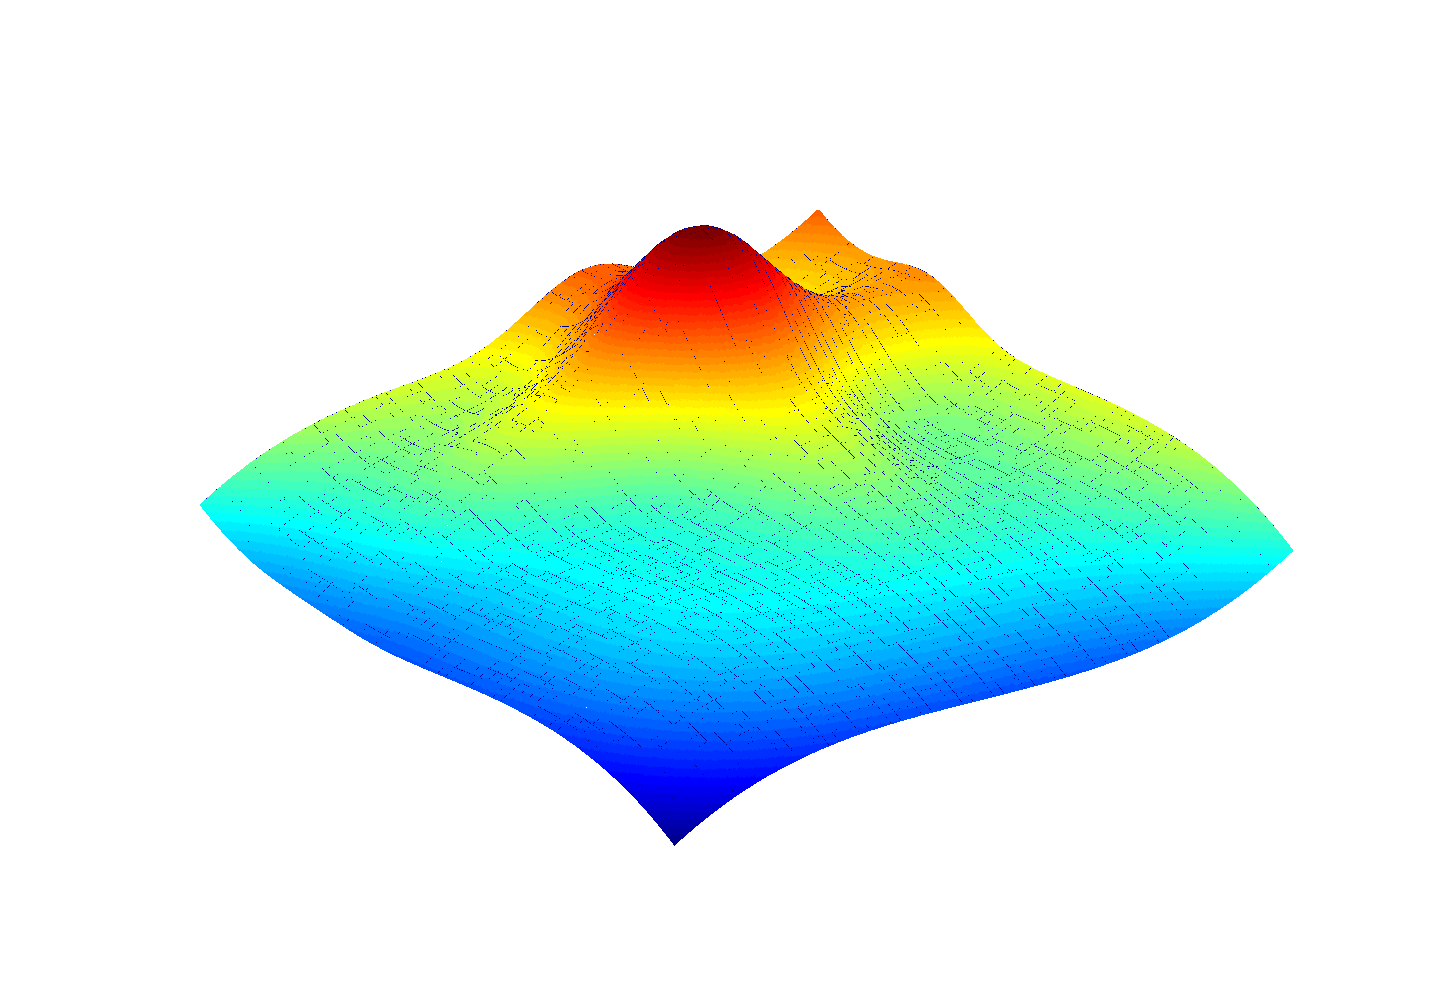
\includegraphics[width=\textwidth]{scalarfieldsource.eps}
%                \caption{Toxic cloud}
%                \label{fig:scalarfieldsource}
%        \end{subfigure}%
%        ~ %add desired spacing between images, e. g. ~, \quad, \qquad etc.
%          %(or a blank line to force the subfigure onto a new line)
%       \caption{Scalar fields} \label{fig:scalar field}
%\end{figure}
%\footnotetext[1]{Picture taken from FeedNetBack project}
%\footnotetext[2]{Picture taken from seaandskyjp.wordpress.com}
%}
% 



\chapter{Dynamic Model of the Quadrotor \label{ch:model}}

In this chapter, the derivation of the quadrotor model is provided. This result
is very important because it describes how the helicopter moves according to its
inputs. Thanks to these equations it is possible to define and predict the positions
reached by the helicopter by investigating just the four motor speeds. The model
equations will be ”inverted” in the next chapter (Control algorithms) to identify
which inputs are needed to reach a certain position.
\\\\
The first section (\fullref{sec:configurations}) shows the main idea of the quadrotor
dynamics and describes intuitively which movements are allowed and how it
manages to perform stationary flight (hovering).
\\\\
The second section () provides the model information
with physics and mathematical derivations. In this work, the Newton-Euler
formalism and the Euler angles theories have been chosen.
\\\\
In the third section (\fullref{sec:nonlinear}), additional information was added to
the model taking into account the whole motor system which is composed of the
motor itself, the reduction gears and the propeller.
\\\\
The last section (\fullref{sec:linearized}) provides an overview of the architecture:
connections between devices and abstraction of the software and task.

\section{Quadrotors Configurations}
\label{sec:configurations}
As the term `quadrotor' refers to a multirotor whose thrust is generated from four motors and propellers, quadrotors can be built in multiple ways as long as they comply with the established definition. There are some configurations that are already standardized being widely used by commercial manufacturers and hobbyists, such as the `+' and `X' configurations.
%\\\\
%\url{https://www.google.com/search?q=why+\%2B+or+x+configuration+quadcopter&ie=utf-8&oe=utf-8&client=firefox-b-ab&gfe_rd=cr&dcr=0&ei=Mr0BWrW9HtHk8AfXm7fADQ}
%\\\\
%\url{https://community.micro-motor-warehouse.com/t/vs-x-configuration/2673}
%\\\\
%\url{https://www.quora.com/Why-is-x-configuration-preferred-over-+-config-of-quadcopter}
%\\\\
%\url{https://www.rcgroups.com/forums/showthread.php?1203569-Quad-X-vs-configuration}


\subsection{`+' Configuration}
The geometry used in quadrotors built in `+' configuration is shown in Fig. \ref{fig:quadcopterplus}.
\\
\begin{figure}[H]
\begin{center}
  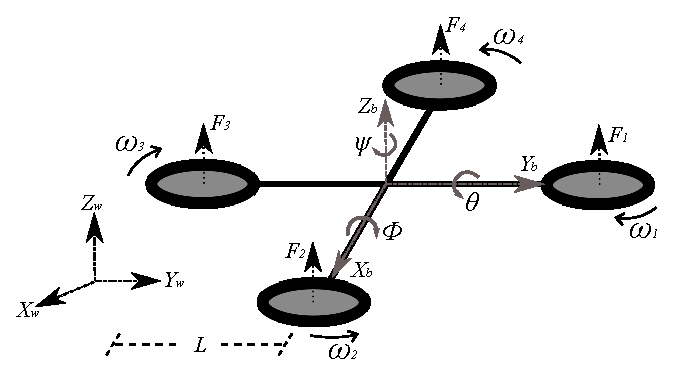
\includegraphics[width=0.90\textwidth]{quadcopterplus.eps}
\caption{Quadrotor geometry in `+' configuration} 
    \label{fig:quadcopterplus}
    \end{center}
\end{figure}
Where, ($\phi$, $\theta$, $\psi$) are the angular deviations (pitch, roll and yaw, respectively) of the quadrotor about the body-frame,
 ($x$, $y$, $z$) are the body-frame axes,  ($X_W$, $Y_W$, $Z_W$) are the earth-frame axes, $L$ is the distance from the quadrotor center of gravity ($CoG$) to the motor center, $F_{M_i}$ is the thrust force exerted by each motor, and $\omega_i$ is the angular velocity of each motor, with $i = 1,2,3,4$. 
\\\\
In this configuration, the body-frame axes $x$ and $y$, coincide with the lines that connect motors of opposite sides in the quadrotor frame. This means that, in order to change the pitch or roll angles, only the angular velocities $\omega_i$ of two motors must be modified, ($\omega_1$, $\omega_3$) for pitch,  and ($\omega_2$, $\omega_4$) for roll, while the generated torques for roll and pitch are applied at a distance of $L$ from the quadrotor $CoG$. Here, $M_1$ is considered as the front motor, $M_3$ as the rear one, $M_2$ as the right motor, and $M_4$ as the left motor. 
\\\\
Even though the quadrotor has 6 DOF, it is equipped just with four propellers, hence it is not possible to reach a desired set-point for all the DOF, but at maximum four. However, thanks to its structure, it is quite easy to chose the four best controllable variables and to decouple them to make the controller easier. The four quadrotor targets are thus related to the four basic movements which allow the helicopter to reach a certain height and attitude. It follows the description of these basic movements.


\subsubsection{Throttle $u$ [$N$]}
\begin{equation}
u = \sum_{i=1}^{4}F_{M_i}
\end{equation}

\subsubsection{Yaw Torque $\tau_{\psi}$ [$N\cdot m$]}
As can be seen in Fig. \ref{fig:quadcopterplus}, $M_1$ and $M_3$ have a clockwise rotation while $M_2$ and $M_4$ rotate counter-clockwise. This configuration of opposite pairs rotational directions allows the system to control its conservation of momentum and thus change its yaw angle in a controlled manner without the need of a tail rotor used in the standard helicopter structure (\cite{Bresciani2008}). In `+' configuration, the fact that the pitch and roll angles are controlled using only two motors that rotate in the same direction, leads to large changes in the thrust force of the other two motors to achieve momentum conservation.
\begin{equation}
\tau_{\psi} = K_{m}(F_{M_2} + F_{M_4} - F_{M_1} - F_{M_3})
\end{equation}

\subsubsection{Roll Torque $\tau_{\theta}$ [$N\cdot m$]}
\begin{equation}
\tau_{\theta} = L(F_{M_4}-F_{M_2})
\end{equation}

\subsubsection{Pitch Torque $\tau_{\phi}$ [$N\cdot m$]}
\begin{equation}
\tau_{\phi} = L(F_{M_3}-F_{M_1})
\end{equation}

\subsubsection{Inputs Setting in `+' Configuration}
\begin{equation}
	U = \begin{bmatrix}
	u\\[5pt]
	\tau_{\psi}\\[5pt]
	\tau_{\theta}\\[5pt]
	\tau_{\phi}
	\end{bmatrix} = \begin{bmatrix}
	1 & 1 & 1 & 1 \\[5pt]
	-K_{m} & K_{m} & -K_{m} & K_{m}\\[5pt]
	0 & -L & 0 & L\\[5pt]
	-L & 0 & L & 0
							\end{bmatrix}
\begin{bmatrix}
F_{M_1}\\[5pt]
F_{M_2}\\[5pt]
F_{M_3}\\[5pt]
F_{M_4}
\end{bmatrix}
	\label{ec:U_X}						
\end{equation}

\subsection{`X' Configuration}
Following the same nomenclature used in the `+' configuration, in `X' configuration, the quadrotor frame is rotated $\pi/4\ rad$ about the $z$-axis in the body-frame, as shown in Fig. \ref{fig:quadrotorX}. 
\\\\
In this case, the front-line in the quadrotor is set between $M_1$ and $M_4$, while $M_2$ and $M_3$ define its back line. Using the `X' configuration, the roll and pitch angles are changed using the forces exerted by all the motors, and not just by two of them. On the other hand, the pitch and roll torques are applied on the axes at a distance $L_X = L\cdot \cos(\pi/4)$. Thereby, the quadrotor has $2\cdot \cos(\pi/4)$ times more available torque to rotate around the $x$ and $y$ axes, when compare with the `+' configuration.

\begin{figure}[H]
\begin{center}
  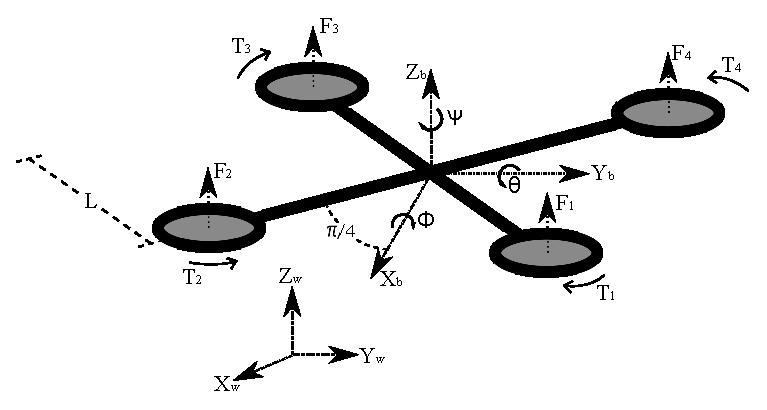
\includegraphics[width=0.97\textwidth]{quadcopter1.eps}
% figure caption is below the figure
\caption{Quadrotor geometry in `X' configuration} 
    \label{fig:quadrotorX}
    \end{center}
\end{figure}

\subsubsection{Throttle $u$ [$N$]}
\begin{equation}
u = \sum_{i=1}^{4}F_{M_i}
\end{equation}

\subsubsection{Yaw Torque $\tau_{\psi}$ [$N\cdot m$]}
\begin{equation}
\tau_{\psi} = K_{m}(F_{M_2} + F_{M_4} - F_{M_1} - F_{M_3})
\end{equation}

\subsubsection{Roll Torque $\tau_{\theta}$ [$N\cdot m$]}
\begin{equation}
\tau_{\theta} = L_{X}(F_{M_3}+F_{M_4}-F_{M_2}-F_{M_1})
\end{equation}

\subsubsection{Pitch Torque $\tau_{\phi}$ [$N\cdot m$]}
\begin{equation}
\tau_{\phi} = L_{X}(F_{M_2}+F_{M_3}-F_{M_1}-F_{M_4})
\end{equation}

\subsubsection{Inputs Setting in `X' Configuration}
$L_{X} = L\cdot \cos\left(\pi/4\right)$ is the real distance between the point of application of the rolling and pitching torques and the quadrotor center of mass along the $x$ and $y$ axes \cite{Faessler2016}.
\\\\
The rolling, pitching and yawing torques contained in vector $\tau$, are generated using the force exerted by each motor as 
\begin{equation}
	U = \begin{bmatrix}
	u\\[5pt]
	\tau_{\psi}\\[5pt]
	\tau_{\theta}\\[5pt]
	\tau_{\phi}
	\end{bmatrix} = \begin{bmatrix}
	1 & 1 & 1 & 1 \\[5pt]
	-K_{m} & K_{m} & -K_{m} & K_{m}\\[5pt]
	-L_{X} & -L_{X} & L_{X} & L_{X}\\[5pt]
	-L_{X} & L_{X} & L_{X} & -L_{X}
							\end{bmatrix}
\begin{bmatrix}
F_{M_1}\\[5pt]
F_{M_2}\\[5pt]
F_{M_3}\\[5pt]
F_{M_4}
\end{bmatrix}
	\label{ec:U_X}						
\end{equation}
where $ T_{i} $ is the torque produced by each motor along the $z_{b}$ axis, $L$ is the distance between each motor rotor and the quadrotor $CoG$, and $L_X$ is the real distance between the point of application of the rolling and pitching torques and the quadrotor $CoG$ along the $x_b$ and $y_b$ axes \cite{Faessler2016}.\\\\



\section{Nonlinear Model}
\label{sec:nonlinear}

This section describes the dynamic modeling used to perform the quadrotor control, based on the study carried out in \cite{modelamiento, modelamientoPDAFC, modelamientoNCQ}. This model represents the quadrotor as a solid symmetrical object subject to a total thrust and three torques, without considering the dynamics of the actuators.


\subsection{Euler-Lagrange Approach}
The general coordinates representing the position and attitude of the quadrotor are defined as
\begin{equation}
	q=\begin{bmatrix}
	\xi & \eta
	\end{bmatrix}^{T},
	\label{ec:coorgenerales}
\end{equation}
where $\xi=\begin{bmatrix}
x & y & z
\end{bmatrix}^{T}$ is the vector representing the position of the center of mass of the quadrotor relative to the body reference frame shown in Fig. \ref{fig:marcoreferencia} and $\eta=\begin{bmatrix}
\psi & \theta & \phi
\end{bmatrix}^{T}$ represent the quadrotor attitude.
\\\\
The Lagrangian of the quadrotor is defined by
\begin{equation}
	L(q,\dot{q})=K_{trans}+K_{rot} - U,	
	\label{ec:lagrangiano}
\end{equation}
where $ K_{trans} = \dfrac{m}{2}\dot{\xi}^{T}\dot{\xi} $ is the translational kinetic energy, $ K_{rot} = \dfrac{1}{2}\dot{\eta}^{T}J\dot{\eta} $ is the rotational kinetic energy, $ U=mgz $ is the potential energy, $m$ is the quadrotor mass , $z$ is the quadrotor elevation, $g$ is the gravity acceleration magnitude, and $J$ is the inertial matrix. The dynamic model of the quadrotor is derived from the Euler-Lagrange equation
\begin{equation}
	\dfrac{d}{dt}\dfrac{\partial L}{\partial \dot{q}}-\dfrac{\partial L}{\partial q}=
	\begin{bmatrix}
	F_{\xi}\\
	\tau
	\end{bmatrix},
	\label{ec:eulerlag}
 \end{equation} 
where $F_{\xi}=R_{b}^{w}\hat{F_{b}}$ is the translational force applied to the quadrotor by the four motors, $\tau$ contains the rolling, pitching and yawing torques, and 
\begin{equation}
R_{b}^{w} = \begin{bmatrix}
C_\theta C_\psi & C_\psi S_\theta S_\phi-C_\phi S_\psi & S_\phi S_\psi+C_\phi C_\psi S_\theta\\
C_\theta S_\psi & S_\psi S_\theta S_\phi+C_\phi C_\psi & C_\phi S_\psi S_\theta - S_\phi C_\psi\\
-S_\theta & C_\theta S_\phi & C_\theta C_\phi
\end{bmatrix}
\end{equation}
is the rotation matrix from the body to the Earth frame where $C_\theta = \cos\theta$ and $S_\theta = \sin\theta$.
\\\\
In the quadrotor body-frame, the translational force $\hat{F_{b}}$ is only applied in the $z_{b}$ axis as shown in Fig. \ref{fig:marcoreferencia}. This force is represented by
\begin{equation}
	\hat{F_{b}}=\begin{pmatrix}
	0\\
	0\\
	u
	\end{pmatrix} = \begin{pmatrix}
	0\\
	0\\
	\sum_{i=1}^{4}F_{M_i}
	\end{pmatrix}  ,
 \label{ec:fuerzas}
 \end{equation} 
with $ F_{M_i} $ being the force, in N, exerted by the motor $ M_{i}$, as shown in Fig. \ref{fig:marcoreferencia}.
\\\\
The force $ F_{M_i} $ has a linear dependency with the square of the motor angular velocity, defined as
\begin{equation}
	F_{M_i}=k_{i}w_{i}^{2},
	\label{ec:fi}
\end{equation}
where $ w_{i} $ is the angular velocity of the motor, and $ k_{i} $ is a proportional constant. However, in practice $F_{M_i}$ must be set using the PWM signal input of an ESC. The thrust-PWM relation is found experimentally and is shown in Section \ref{sec:Implementation}.
\\\\
The Euler-Lagrange equations can be divided in two parts, one for the $\xi$ coordinates and another for the $\eta$ coordinates, getting
\begin{equation}
\label{eqn:E-L1}
\ddot{\xi} =
\begin{bmatrix}
\ddot{x} \\ \ddot{y} \\ \ddot{z}
\end{bmatrix} 
=
\begin{bmatrix}
\frac{u_{1}}{m}(C_\phi S_\theta C_\psi + S_\phi S_\psi) \\
 \frac{u_{1}}{m}(C_\phi S_\theta S_\psi - S_\phi C_\psi) \\
\frac{u_{1}}{m}(C_\phi C_\theta) - g
\end{bmatrix},
\end{equation}
\begin{equation}
\label{eqn:E-L2}
\ddot{\eta} =
\begin{bmatrix}
\ddot{\psi} \\ \ddot{\theta} \\ \ddot{\phi}
\end{bmatrix} 
 =
\begin{bmatrix}
\dot{\phi}\dot{\theta}\dfrac{J_{xx}-J_{yy}}{J_{zz}} + \dfrac{u_{2}}{J_{zz}} \\
\dot{\phi}\dot{\psi}\dfrac{J_{zz}-J_{xx}}{J_{yy}} + \dfrac{u_{3}}{J_{yy}} \\
 \dot{\theta}\dot{\psi}\dfrac{J_{yy}-J_{zz}}{J_{xx}} +  \dfrac{u_{4}}{J_{xx}}
\end{bmatrix},
\end{equation}
where, $\begin{bmatrix}
u_{1},\ u_{2},\ u_{3}, \ u_{4}
\end{bmatrix}^{T} = \begin{bmatrix}
u,\ \tau_{\psi},\ \tau_{\theta},\ \tau_{\phi}
\end{bmatrix}^{T} $, and $ (J_{xx}, J_{yy}, J_{zz}) $ are the moments of inertia around the quadrotor body-frame axes \cite{Emam2016, Badr2016}.
\\\\

that is a simplified representation of the quadrotor complete model found in \cite{Bouabdallah2007}.

\subsection{Newton-Euler Approach}
sdasdasdaasd

\section{Linearized Model}
\label{sec:linearized}
\setcounter{MaxMatrixCols}{20}
\subsection{Jacobian Linearization}
\cite{Sabatino2015}
\\\\
The Euler-Lagrange equations in (\ref{eqn:E-L1}) and (\ref{eqn:E-L2}) are linearized using their Jacobian around the hover state where $\begin{bmatrix}
\eta,\ \dot{\eta},\ \dot{\xi}
\end{bmatrix} \to \begin{bmatrix}
0,\ 0,\ 0
\end{bmatrix}$, getting
\begin{equation}
\label{eqn:linear}
\ddot{q}
=
\begin{bmatrix}
g\theta \\
g\phi\\
u_{1}/m \\
u_{2}/J_{zz} \\
u_{3}/J_{yy} \\
u_{4}/J_{xx}
\end{bmatrix},
\end{equation}

As said above, in order to perform the linearization, an equilibrium point is
needed. Such an equilibrium point can be:
\begin{equation}
\overline{\mathbf{x}} = \begin{bmatrix}
\overline{x} & \overline{y} & \overline{z} & 0 & 0 & 0 & 0 & 0 & 0 & 0 & 0 & 0
\end{bmatrix}^{T}
\end{equation}
From the equations, we can find that the equilibrium point (2.29) is obtained by
the constant input value:
\begin{equation}
\overline{\mathbf{u}} = \begin{bmatrix}
mg & 0 & 0 & 0
\end{bmatrix}^{T}
\end{equation}
with $mg$ being the lift force.
\\\\
The linearized model of the quad-rotor helicopter written as a state space model is given by

\begin{align*}
\dot{\mathbf{x}}(t) = & A\mathbf{x}(t)+B\mathbf{u}(t),\\
\mathbf{y}(t) = & C\mathbf{x}(t),
\end{align*}
where
\begin{align}
\begin{split}
A  = \frac{\partial f(\mathbf{x},\mathbf{u})}{\partial \mathbf{x}}\Bigr|_{\substack{\mathbf{x}=\overline{\mathbf{x}}\\\mathbf{u}=\overline{\mathbf{u}}}} = & 
\begin{bmatrix}
0 & 1 & 0 & 0 & 0 & 0 & 0 & 0 & 0 & 0 & 0 & 0\\[2px]
0 & 0 & 0 & 0 & 0 & 0 & 0 & 0 & g & 0 & 0 & 0\\[2px]
0 & 0 & 0 & 1 & 0 & 0 & 0 & 0 & 0 & 0 & 0 & 0\\[2px]
0 & 0 & 0 & 0 & 0 & 0 & 0 & 0 & 0 & 0 & g & 0\\[2px]
0 & 0 & 0 & 0 & 0 & 1 & 0 & 0 & 0 & 0 & 0 & 0\\[2px]
0 & 0 & 0 & 0 & 0 & 0 & 0 & 0 & 0 & 0 & 0 & 0\\[2px]
0 & 0 & 0 & 0 & 0 & 0 & 0 & 1 & 0 & 0 & 0 & 0\\[2px]
0 & 0 & 0 & 0 & 0 & 0 & 0 & 0 & 0 & 0 & 0 & 0\\[2px]
0 & 0 & 0 & 0 & 0 & 0 & 0 & 0 & 0 & 1 & 0 & 0\\[2px]
0 & 0 & 0 & 0 & 0 & 0 & 0 & 0 & 0 & 0 & 0 & 0\\[2px]
0 & 0 & 0 & 0 & 0 & 0 & 0 & 0 & 0 & 0 & 0 & 1\\[2px]
0 & 0 & 0 & 0 & 0 & 0 & 0 & 0 & 0 & 0 & 0 & 0
\end{bmatrix}, \\[15px]
B = \frac{\partial f(\mathbf{x},\mathbf{u})}{\partial \mathbf{u}}\Bigr|_{\substack{\mathbf{x}=\overline{\mathbf{x}}\\\mathbf{u}=\overline{\mathbf{u}}}} = & 
\begin{bmatrix}
0 & 0 & 0 & 0 & 0 & \frac{1}{m} & 0 & 0 & 0 & 0 & 0 & 0\\[5px]
0 & 0 & 0 & 0 & 0 & 0 & 0 & \frac{1}{I_{zz}} & 0 & 0 & 0 & 0\\[5px]
0 & 0 & 0 & 0 & 0 & 0 & 0 & 0 & 0 & \frac{1}{I_{yy}} & 0 & 0\\[5px]
0 & 0 & 0 & 0 & 0 & 0 & 0 & 0 & 0 & 0 & 0 & \frac{1}{I_{xx}}
\end{bmatrix}^{T},\\[15px]
C = &
\begin{bmatrix}
1 & 0 & 0 & 0 & 0 & 0 & 0 & 0 & 0 & 0 & 0 & 0\\
0 & 0 & 1 & 0 & 0 & 0 & 0 & 0 & 0 & 0 & 0 & 0\\
0 & 0 & 0 & 0 & 1 & 0 & 0 & 0 & 0 & 0 & 0 & 0\\
0 & 0 & 0 & 0 & 0 & 0 & 1 & 0 & 0 & 0 & 0 & 0 
\end{bmatrix},
\end{split}
\end{align}

with the parameters  

$m=0.64 $ kg, 

$g=9.81$ m/s.


The state vector is defined as

\begin{align*}
x(t)=&
\begin{bmatrix}
r_x & \dot{r}_x & r_y & \dot{r}_y & r &\dot{r}_z 
\end{bmatrix}^T,
\end{align*}
and the control inputs as
\begin{align*}
u(t)=&
\begin{bmatrix}
u_1 & u_2 &u_3 & u_4
\end{bmatrix}^T,
\end{align*}

and the output vector is defined as

\begin{align*}
r(t)=
\begin{bmatrix}
r_{x} & r_{y} & r_{z}
\end{bmatrix}^T.
\end{align*}

\subsection{Thrust Compensation}
\url{https://robotics.stackexchange.com/questions/4247/tilt-compensated-motor-output-to-keep-altitude-for-quadcopter}
Recalling the rotation matrix $R_{b}^{w}$,
\begin{equation}
R_{b}^{w} = \begin{bmatrix}
c\theta c\psi & c\psi s\theta s\phi-c\phi s\psi & s\phi s\psi+c\phi c\psi s\theta\\
c\theta s\psi & s\psi s\theta s\phi+c\phi c\psi & c\phi s\psi s\theta - s\phi c\psi\\
-s\theta & c\theta s\phi & c\theta c\phi
\end{bmatrix}
\end{equation}
\begin{equation}
u = u^{*} \cos{\theta}\cos{\phi}
\end{equation}
\begin{equation}
u^{*} = \dfrac{u}{\cos{\theta}\cos{\phi}}
\end{equation}
\section{Conclusions}
This chapter presented the design of the two vehicles developed in this thesis.
The test-bench and the OS4. The first system is only capable of 3 DoF which
facilitates the testing of the controllers. However, it is possible to detach the
flying part in order to test free flights. Before designing the second system
which is a free flying quadrotor, a new design methodology is introduced. It
allows an optimal design of small-scale rotorcraft. Four new design indicators
were introduced for a precise and complete evaluation of the design performance.
This methodology appreciably facilitated the components selection
process and battery dimensioning of OS4. This quadrotor exhibits higher
capabilities and endurance than the competition. This is verified through
the comparison of different design parameters. OS4 embeds all the necessary
avionics and energy devices for a fully autonomous flight. This comprises a
low cost IMU, a vision based position sensor specifically developed for this
project and an obstacle detection setup.


\chapter{Smartphone-based Quadrotor Prototype} \label{ch:prototype}
In this chapter, the quadrotor prototype is presented. All the components that are used to build the prototype are described with the purpose of detailing the function that each component fulfils within the quadrotor. Furthermore, the specific parameters of the built quadrotor are shown and the procedure carried out to find them experimentally is explained. This is of great importance for the design of the controllers that allow the flight of the built system.
\\\\
In Fig. \ref{fig:hardwareoverview}, a small overview of the hardware related to the electrical signals within the quadrotor is presented. This overview shows the interrelation between the main components detailed below.
\begin{figure}[h]
	\begin{center}
		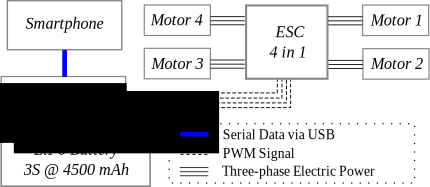
\includegraphics[width=13.0cm]{hardwareOverview}    
		\caption{Quadrotor prototype's hardware overview} 
		\label{fig:hardwareoverview}
	\end{center}
\end{figure}

\section{Quadrotor Components}
\label{sec:components}
The hardware used to build the quadrotor prototype is detailed in this section. The main goal of this research project is to control a quadrotor using just a smartphone on-board. This smartphone executes the state estimation algorithms and defines the controls signals that will command the actuators. The control signals are processed in the smartphone and then sent, through a gateway, to the Electronic Speed Controllers (ESCs) that will set the angular speed of the motors depending on the control signal they receive.
\subsection{Frame}
The quadrotor's frame is responsible for carrying all the other components needed in the system. Additionally, it must be able to support the weight of any possible payload that the quadrotor will carry. The multirotors frames are usually built using fiberglass or carbon fiber as main material, being the carbon fiber frames stiffer and lighter than equally built fiberglass frames.
\\\\
For this project, the requirement to build a quadrotor between $0.20$ and $0.30\ cm$ in radius was defined. This requirement is based on the fact that the quadrotor must carry a smartphone and possibly some mission-related payloads, which weight can be greater than $100\ g$. Taking that requirement and the literature review into account, in addition to the weight and stiffness advantages of the carbon fiber, a LJI 500-X4 carbon fiber frame was selected.
\begin{figure}[h]
\begin{center}
\includegraphics[width=8.6cm]{lji500x4.jpg}    
\caption[LJI 500-X4 carbon fiber frame]{LJI 500-X4 carbon fiber frame\protect\footnotemark} 
\label{fig:quadframe}
\end{center}
\end{figure}
\footnotetext{LJI 500-X4 frame image taken from \url{https://goo.gl/hHfHQR}}
\\
This frame (Fig. \ref{fig:quadframe}) has a weight of $431\ g$ and a radius $L$ of $0.244\ m$ measured between the frame center and each of the four rotor axis holes. Its landing gear has a height of $0.170\ m$, allowing the payload to be placed in the lower part of the quadrotor.

\subsection{Smartphone}
In this project, the smartphone takes the place of the quadrotor's flight controller. The basic instrumentation needed for a flight controller includes a triaxial accelerometer, a triaxial gyroscope, a triaxial magnetometer, a barometer and a GNSS receiver that can process signals from the GPS and GLONASS satellites constellations. On the other side, the processor of a flight controller must be powerful enough to execute the control and estimation algorithms within the sample time of the control system.
\\\\
The LG Nexus 5X, shown in Fig. \ref{fig:nexus}, is a smartphone developed by Google and assembled by LG, released in 2015 with the Android 6.0.1 operating system. This phone has a Hexa-core Qualcomm MSM8992 Snapdragon 808 CPU that includes four Cortex-A53 and two Cortex-A57 cores with 1.4 GHz and 1.8 GHz clock rate respectively and an Adreno 418 GPU. Its features also include 2 GB of RAM memory, 32 GB of Flash memory, total mass of 136 g and a 12.3 MP camera.
\\
\begin{figure}[H]
\begin{center}
\includegraphics[width=5.5cm]{nexus5x.jpg}    
\caption[LG Nexus 5X, smartphone used as flight controller]{LG Nexus 5X, smartphone used as flight controller\protect\footnotemark} 
\label{fig:nexus}
\end{center}
 \end{figure}
 \footnotetext{LG Nexus 5X image taken from \url{https://goo.gl/RxyDJd}}
 \vspace{-0.5cm}
This smartphone features all the needed instrumentation for a flight controller, specified previously. The maximum sample rates of the instrumentation contained in the LG Nexus 5X are described in Table \ref{tb:samplerates}.
\begin{table}[h]
\small
\begin{center}
\caption{Sample Rates of the Sensors in the Smartphone}\label{tb:samplerates}
\begin{tabular}{c|c}\hline
\rule{0pt}{3ex} Sensor & Sample rate $[Hz]$ \\\hline\hline
\rule{0pt}{3ex}Triaxis accelerometer &  $400$ \\[0.7ex]
Triaxis gyroscope &  $200$ \\[0.7ex]
Triaxis magnetometer & $50$ \\[0.7ex]
Barometer &  $10$ \\[0.7ex] 
GNSS &  $1$  \\[0.7ex]\hline
\end{tabular}
\end{center}
\end{table}
\\\\
The LG Nexus 5X smartphone was selected in this project mainly due to its computational and instrumentation capabilities in addition to its communication interfaces (Bluetooth 4.0, Wireless LAN, USB Type-C and GSM). Its powerful CPU handling a GPU enables the possibility of developments using the camera for visual odometry, and controllers whose execution represents a high computational load, which exceeds the limits of a standard microcontroller such as the ATmega 2560.
\\\\
As the quadrotor's flight controller, the smartphone receives remote orders from the quadrotor's pilot using wireless communication, while executing the sensorial, estimation and control algorithms. After the control signals are calculated, they are sent to the actuators as a serial data frame using the USB interface between the smartphone and a gateway that converts the serial data into PWM signals.

\subsection{Motors and Electronic Speed Controllers}
The actuation system of the quadrotor is composed by R/C-type brushless motors, propellers and ESCs. The LJI 500-X4 frame manufacturer recommends using motors with a RPM constant of $810\ KV$, which means that these motors can rotate at a speed of $810\ RPM$ for each Volt applied to it. This kind of motors are used in medium to big sized multirotors due to its thrust efficiency and thrust capacity.
\\\\
Following this recommendation, the EMAX MT2216II motors were selected. These motors, shown in Fig. \ref{fig:emaxmotor}, are labelled by its manufacturer as $810\ KV$ motors with a maximum current consumption of $9.8\ A$ and a maximum thrust of $6.6\ N$, when using a $10$-inch propeller.
\begin{figure}[H]
\begin{subfigure}{.5\linewidth}
\centering
\includegraphics[width=5.6cm]{emax2216II2.png}    
\caption{EMAX MT2216II motor} 
\label{fig:emaxmotor}
\end{subfigure}
\begin{subfigure}{.5\linewidth}
\centering
\includegraphics[width=7.0cm]{emax4in1.jpg}    
\caption{EMAX 4in1 ESC} 
\label{fig:emaxESC}
\end{subfigure}
\caption{Motors and ESC used in the Quadrotor\protect\footnotemark}
\label{fig:motorandesc}
\end{figure}
\footnotetext{Taken from \url{https://goo.gl/6qD6Qg} and \url{https://goo.gl/fDHiUp}}
The quadrotor's brushless motors are powered using a three-phase electric signal generated by the ESC. Each ESC sets one motor rotational velocity depending on a PWM signal input, and must be able to handle the maximum current consumption of the motor. Mainly due to the ease of handling and positioning within the frame, the EMAX 4in1 ESC was selected for this project (Fig. \ref{fig:emaxESC}). This 4in1 ESC contains four ESCs with a maximum current supply of $30\ A$ each. It also has a DC-DC converter that outputs an isolated $5\ V$ DC supply for any additional electronics. The power supply of the ESC is fully delivered by the quadrotor's battery.

\subsection{Smartphone-to-ESC Gateway}
As the smartphone can not generate any PWM signal and each ESC needs a PWM signal input to set the rotational velocity of a motor, a gateway between the smartphone and the ESCs must be used. In order to avoid interference in the electromagnetic spectrum and delays that could lead the control system to instability while using wireless communications, the smartphone wired serial bus (USB interface) is defined as the only channel of communication through which the control signals are sent to the gateway.
\\\\
The Arduino Mega ADK, is shown in Fig. \ref{fig:megaadk}, is a development board based on the Atmel 8-bit AVR RISC-based ATmega2560 microcontroller.  This board supports the Android Open Accesory (AOA) protocol, which allows external hardware to exchange data with Android devices.
\begin{figure}[H]
\begin{center}
\includegraphics[width=7.6cm]{megaADK.jpg}    
\caption[Arduino Mega ADK]{Arduino Mega ADK\protect\footnotemark} 
\label{fig:megaadk}
\end{center}
 \end{figure}
 \footnotetext{Arduino Mega ADK image taken from \url{https://goo.gl/ejeQeX}}
\vspace{-0.5cm}
Although there are other boards that support the AOA protocol, as the IOIO board, the Arduino Mega ADK offers the possibility of executing tasks in the ATmega2560 microcontroller without any intervention of the Android device. This feature is very useful in case of future developments that include additional hardware to the smartphone-based quadrotor.
\\\\
The Arduino Mega ADK is selected as the smartphone-to-ESC gateway. The workflow of this board is set as follows: the microcontroller receives a serial data frame from the smartphone through the USB port, each of the four PWM signal widths is extracted from the data frame, the PWM signals are sent to the ESCs, finally the cycle starts again. This workflow is executed each $2\ ms$ and if the gateway does not receive any updated data frame from the smartphone, it keeps the last PWM signals set.

\subsection{Battery}
The quadrotor's battery must supply power to all the active components in the quadrotor. The maximum power consumption of these components, based on the nominal voltage value of a 3-cells lithium-ion polymer (LiPo) battery ($11.1\ V$), is shown below.\\
\begin{table}[h]
\small
\begin{center}
\caption{Maximum Power Consumption of the Quadrotor's Components}\label{tb:power}
\begin{tabular}{c|c|c|c}\hline
\rule{0pt}{3ex} Component & Voltage $[V]$ & Max. Current $[A]$ & Max. Power $[W]$ \\\hline\hline
\rule{0pt}{3ex}
Smartphone &  $5$ & $0.75$ & $3.75$ \\[0.4ex]
Arduino Mega ADK & $11.1$ & $0.75$ & $8.33$ \\[0.4ex] 
4 x ESCs &  $11.1$ & $1.38$ & $15.32$ \\[0.4ex]
4 x Motors & $11.1$ & $39.2$ & $435.12$ \\[0.4ex]\hline
\end{tabular}
\end{center}
\end{table}
\vspace{-0.5cm}
\\The maximum current consumption in the quadrotor reaches $42.08\ A$, so the battery must be able to deliver current amplitudes greater than that value. A Floureon 3-cells LiPo battery with a nominal capacity of $4500\ mAh$ and a nominal voltage of $11.1\ V$, was selected for this prototype and is shown in Fig. \ref{fig:battery}. This battery can deliver up to $30$ times its nominal current, this is $135\ A$, continuously.
\begin{figure}[H]
	\begin{center}
		\includegraphics[width=9.0cm]{floureon.jpg}    
		\caption[LiPo battery that powers the Quadrotor]{LiPo battery that powers the Quadrotor\protect\footnotemark} 
		\label{fig:battery}
	\end{center}
\end{figure}
\footnotetext{Floureon 3S LiPo battery image taken from \url{https://goo.gl/anC9M2}}

\subsection{3D-printed Parts}
The smartphone, the Arduino Mega ADK and the 4in1 ESC need to be easily placed and protected when installed on the frame. For that reason, multiple support components and one case were designed and 3D-printed using polylactic acid (PLA) filament. These 3D-printed objects are detailed below.

\subsubsection{Smartphone Support}
In order to place the smartphone near the $CoG$ in the quadrotor and enable the possibility of capturing nadir photos or videos, the smartphone support is designed in such a way that it can be placed under the quadrotor's $CoG$ but above the landing gear of the frame. Additionally, the support includes a free area that allows to use the complete field of view of the camera without being obstructed by it. The smartphone support is shown in Fig. \ref{fig:phonesupport}.
\begin{figure}[h]
	\begin{center}
		\includegraphics[width=8.6cm]{phonesupport2.png}    
		\caption{Smartphone support} 
		\label{fig:phonesupport}
	\end{center}
\end{figure}
\vspace{-0.5cm}
\subsubsection{Arduino Mega ADK and ESC supports}
The Arduino Mega ADK and the Emax 4in1 ESC are placed on the frame, above the quadrotor's $CoG$. Given the limited space available to locate these components on the top of the frame, their supports are designed to be placed one on top of the other, as shown in Fig. \ref{fig:megaandescsupports}.
\begin{figure}[h]
\begin{subfigure}{.5\linewidth}
\centering
\includegraphics[width=7.0cm]{megasupport2.png}
\caption{Arduino Mega ADK support} 
\label{fig:megasupport}
\end{subfigure}%
\begin{subfigure}{.5\linewidth}
\centering
\includegraphics[width=7.0cm]{escsupport2.png}
\caption{ESCs support} 
\label{fig:escsupport}
\end{subfigure}\\[1ex]
\begin{subfigure}{\linewidth}
\centering
\includegraphics[width=7.0cm]{megaandescsupport2.png}
\caption{Arrangement of the Gateway and ESCs Support as a Whole} 
\label{fig:megaandescsupport}
\end{subfigure}
\caption{Arduino Mega ADK and EMAX 4in1 ESCs designed supports}
\label{fig:megaandescsupports}
\end{figure}

\subsubsection{Dome}
To protect the Arduino Mega ADK and the ESCs, a dome that covers and encloses them is designed. This dome, shown in Fig. \ref{fig:dome}, totally encloses the Mega ADK and ESCs supports restricting their movement and protecting them in case of a shock or hit.
\begin{figure}[H]
	\begin{center}
		\includegraphics[width=8.6cm]{dome2.png}    
		\caption{3D Designed Dome} 
		\label{fig:dome}
	\end{center}
\end{figure}

\subsection{Assembled Smartphone-based Quadrotor}
The smartphone-based quadrotor prototype is assembled using all the components exposed in this section, and is shown in Fig. \ref{fig:completequad}.
\begin{figure}[H]
	\begin{center}
		\includegraphics[width=14cm]{complete.jpg}    
		\caption{Assembled Smartphone-based Quadrotor Prototype} 
		\label{fig:completequad}
	\end{center}
\end{figure}

\section{Quadrotor Parameters} \label{sec:parameters}
In this section, the quadrotor parameters are detailed. These parameters define the specific dynamic model for the smartphone-based quadrotor prototype and the conversion of control signals to correctly set the motors thrust.
\subsection{Mass}
The mass of each quadrotor's component is measured using a kitchen scale that has an uncertainty of $\pm 1\ g$. The results are shown in Table \ref{tb:mass}.
\begin{table}[h]
\small
\begin{center}
\caption{Mass values of all the Quadrotor's components}\label{tb:mass}
\begin{tabular}{c|c}\hline
\rule{0pt}{3ex} Component & Mass $[kg]$ \\\hline\hline
\rule{0pt}{3ex}Smartphone &  $0.136$ \\[0.7ex]
Frame &  $0.431$ \\[0.7ex]
Battery & $0.351$ \\[0.7ex]
ESC &  $0.110$ \\[0.7ex] 
Arduino Mega ADK &  $0.330$ \\[0.7ex]
Motors (4) & $0.140$ \\[0.7ex]
Propellers (4) &  $0.380$ \\[0.7ex]
Smartphone support &  $0.105$ \\[0.7ex]
ADK support &  $0.590$  \\[0.7ex]
ESC support &  $0.350$  \\[0.7ex]
Dome &  $0.130$ \\[0.7ex]\hline
\rule{0pt}{3ex} Total & $1.568$
\end{tabular}
\end{center}
\end{table}
\\\\The total mass of the quadrotor $m$ is then calculated as the sum of the weight of each of the components in the quadrotor, being $m = 1.568\ kg$.
\subsection{Moments of Inertia}
As exposed by \cite{Lee2011}, in a quadrotor, the moment of inertia matrix $J$ is set as
\begin{equation}
J = \begin{bmatrix}
J_{xx} & -J_{xy} & -J_{xz} \\
-J_{yx} & J_{yy} & -J_{yz} \\
-J_{zx} & -J_{zy} & J_{zz}
\end{bmatrix}.
\end{equation}
Taking into account that the quadrotor's symmetry with respect to the $x$ and $y$ axes is assumed, the $J$ matrix can be approximated to
\begin{equation}
J  	\approx  \begin{bmatrix}
J_{xx} & 0 & 0 \\
0 & J_{yy} & 0 \\
0 & 0 & J_{zz}
\end{bmatrix}.
\end{equation}
The $J_{xx}$, $J_{yy}$ and $J_{zz}$ values can be obtained using multiple methods including: using a CAD model of the quadrotor and obtaining the inertia values from a 3D design software (\cite{Khodja2017}), approximating the shape of the quadrotor components to cylinders, cubes and other basic shapes to simplify the mathematical calculation of inertia (\cite{Tomas2011}), and developing the bifilar pendulum experiment on the quadrotor (\cite{Garcia2017}). For this project, it was decided to obtain the quadrotor parameters experimentally, so the bifiliar pendulum experiment was developed.
\\\\
In the bifilar pendulum experiment, an object is hung from two parallel ropes of length $r$ and separated by a distance $2l$, being allowed to rotate freely around a the axis that is parallel to the ropes. In Fig. \ref{fig:bifilar}, the geometry of the experiment to get  $J_{zz}$, is shown. For the $J_{xx}$ and $J_{yy}$ inertias experiment, it is necessary to place the quadrotor hanging in such a way that the $x$ and $y$ axes are pointing paraller to the ropes, respectively.
\begin{figure}[h]
	\begin{center}
		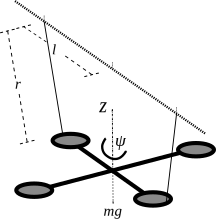
\includegraphics[width=6.0cm]{quadrotorInertia1}    
		\caption{Bifilar pendulum experiment geometry for inertia identification} 
		\label{fig:bifilar}
	\end{center}
\end{figure}
\\Once the quadrotor is hanging from the ropes, a small torque is applied manually to the quadrotor making it rotate about the vertical axis. The tension in the ropes makes the quadrotor swing, with a period of $T_{osc}$ [$s$], about the rotation axis.
\\\\
The moment of inertia is then calculated using the bifiliar equation
\begin{equation}
J.. = \dfrac{m|\vec{g}|T_{osc}^{2}l^{2}}{4\pi^{2}r}\ [kg\cdot m^{2}],
\end{equation}
where $m = 1.568\ kg$ is the quadrotor's total mass and $|\vec{g}| = 9.807\ m/s^{2}$ is the gravity acceleration magnitude (\cite{Mustapa2016}).
\\\\
In Fig. \ref{fig:inertiatest}, it is shown the excursion of the rotation angles, $\phi$, $\theta$ and $\psi$, about the $x$, $y$ and $z$ axes respectively, while performing the bifilar pendulum experiment separately.
\begin{figure}[H]
\begin{subfigure}{.5\linewidth}
\centering
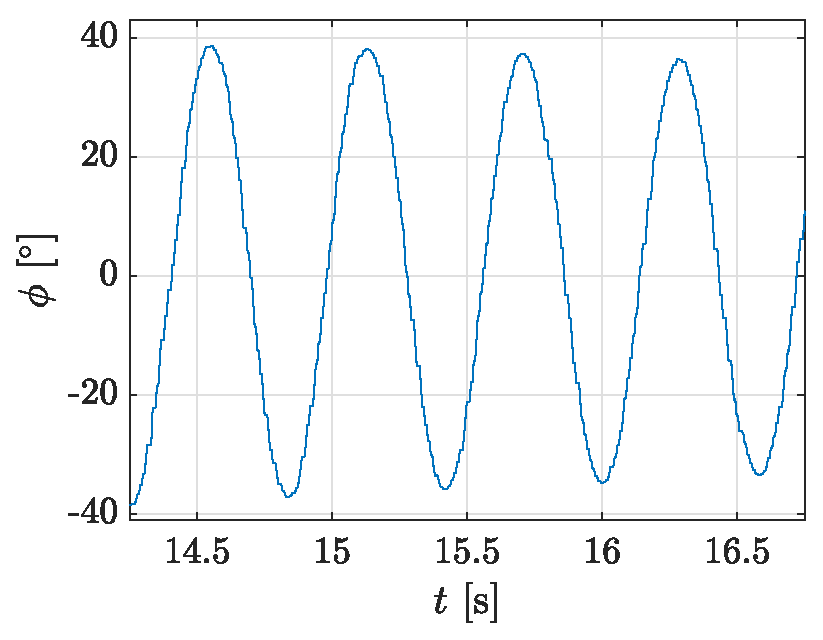
\includegraphics[width=7.0cm]{Ixx}
\caption{Rotation about $x$ axis, $J_{xx}$ experiment}
\label{fig:Jxx}
\end{subfigure}%
\begin{subfigure}{.5\linewidth}
\centering
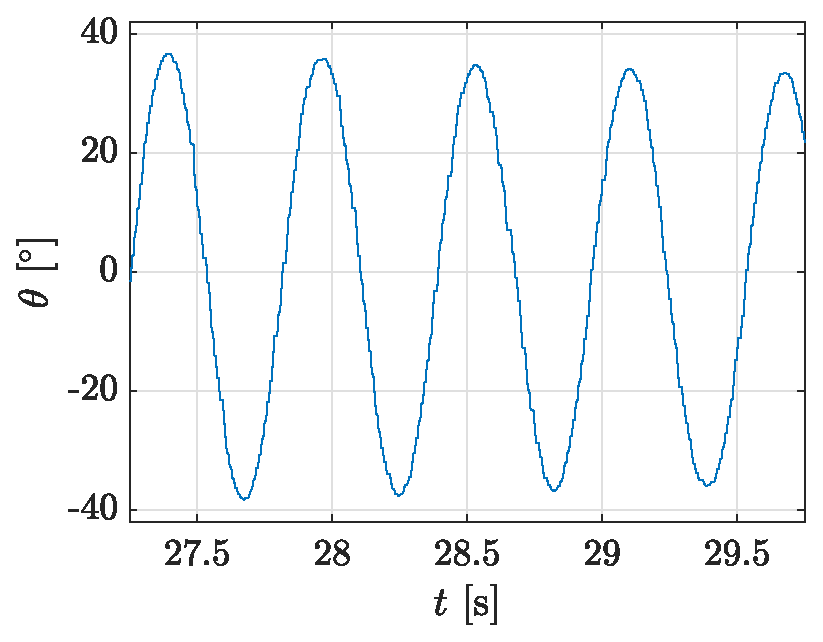
\includegraphics[width=7.0cm]{Iyy}
\caption{Rotation about $y$ axis, $J_{yy}$ experiment}
\label{fig:Jyy}
\end{subfigure}\\[1ex]
\begin{subfigure}{\linewidth}
\centering
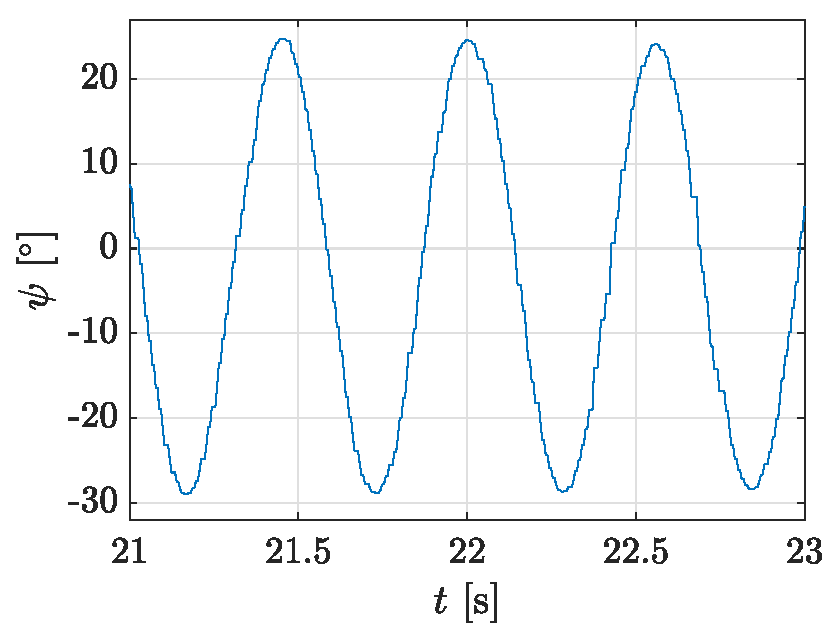
\includegraphics[width=7.0cm]{Izz}
\caption{Rotation about $z$ axis, $J_{zz}$ experiment}
\label{fig:Jzz}
\end{subfigure}
\caption{Rotation about $x$, $y$ and $z$ axes during the bifilar pendulum experiments}
\label{fig:inertiatest}
\end{figure}
The resulting data got after the execution of the experiment around the three components of the quadrotor body frame, are shown in Table \ref{tb:inertiaexperiment}.
\begin{table}[H]
\small
\begin{center}
\caption{Bifilar pendulum experiment results}\label{tb:inertiaexperiment}
\begin{tabular}{c|c|c|c|c}\hline
\rule{0pt}{3ex} Rotation Axis & $r$ [$m$] & $l$ [$m$] & $T_{osc}$ [$s$] & Inertia value [$kg\cdot m^{2}$] \\\hline\hline
\rule{0pt}{3ex} $x$ &  $1.18$ & $0.173$ & $1.168$ & $J_{xx} = 0.0135$ \\[0.7ex]
$y$ &  $1.10$ & $0.173$ & $1.080$ & $J_{yy} = 0.0124$ \\[0.7ex]
$z$ &  $1.025$ & $0.265$ & $1.122$ & $J_{zz} = 0.0336$ \\[0.7ex]\hline
\end{tabular}
\end{center}
\end{table}

\subsection{Motors Thrust}
As seen in Section \ref{sec:components}, the motors rotational velocity $\omega_{i}$ is set by the ESC, which receives a $PWM$ signal input. However, the inputs of the quadrotor ($u$, $\tau_\psi$, $\tau_\theta$, and $\tau_\phi$) depend on the thrust force $F_{M_{i}}$ applied by each quadrotor motor, as exposed in Section \ref{sec:inputsetting}.
\\\\
In order to correctly set the desired force $F_{M_{i}}$ in each motor during a flight, it is necessary to characterize the motor; and thus know how the force applied by the motor behaves with respect to the input $PWM$ signal. This characterization is carried out by means of a thrust test.
\\\\
In the thrust test, the motor and its corresponding propeller are fixed pointing up over a calibrated scale, as shown in Fig. \ref{fig:thrusttest}, while connected to the ESC, and then the \textit{PWM} signal is increased with steps of $10$, with $0$ being the minimum width of \textit{PWM} signal and $255$ the maximum, until reaching the maximum \textit{PWM} width. 
\begin{figure}[h]
	\begin{center}
		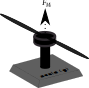
\includegraphics[width=7.0cm]{thrustTest}    
		\caption{Thrust test configuration} 
		\label{fig:thrusttest}
	\end{center}
\end{figure}
\\With each  \textit{PWM} signal width increment, a scale reading is made. Since the readings $m_{s}$ are obtained in units of mass ($kg$), the $F_{M_i}$ must be calculated as
\begin{equation}
F_{M_i} = m_{s}|\vec{g}|\ [N].
\end{equation}
This test was developed twice with each motor and its results are shown in Fig. \ref{fig:motor}.
\begin{figure}[H]
\begin{subfigure}{.5\linewidth}
\centering
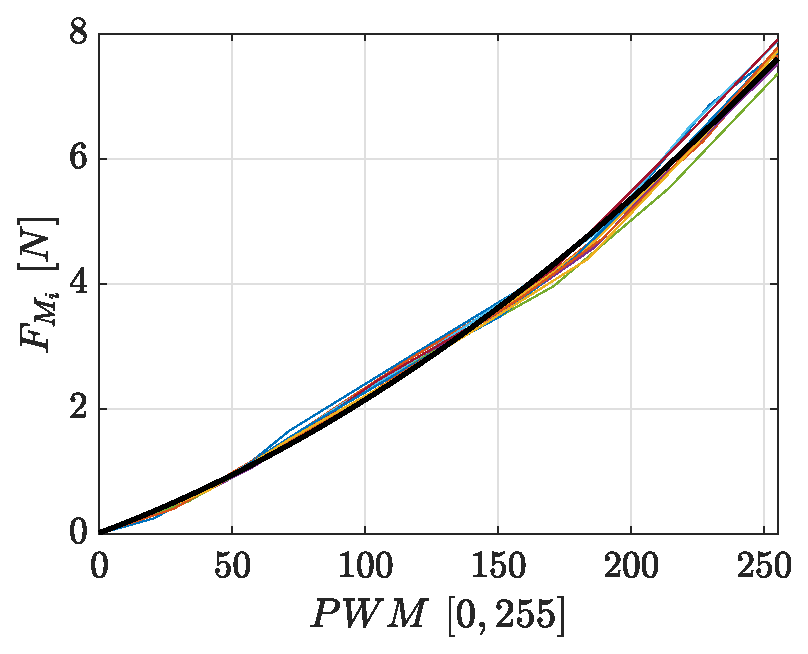
\includegraphics[width=7.0cm]{motorNvsPWM}
\caption{Motors characterization}
\label{fig:motor}
\end{subfigure}%
\begin{subfigure}{.5\linewidth}
\centering
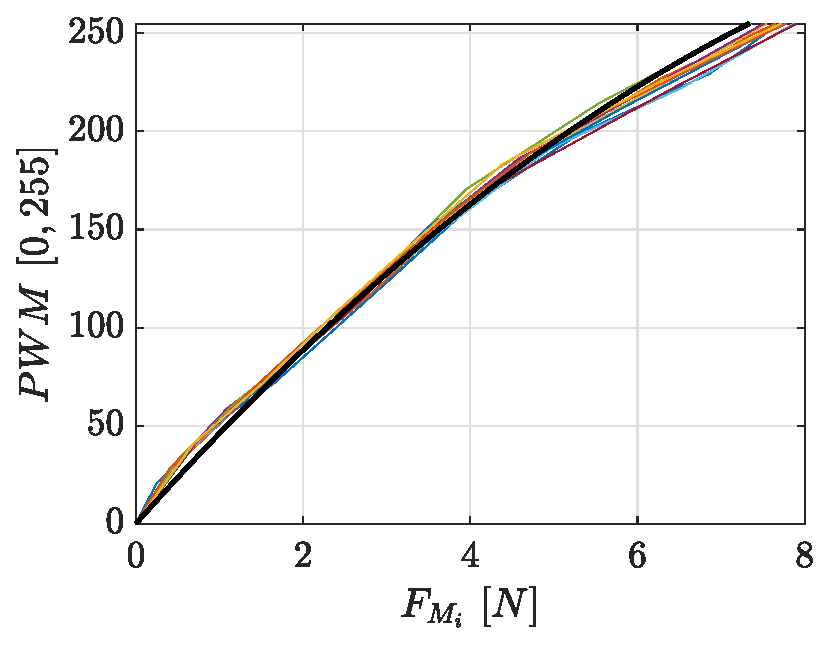
\includegraphics[width=7.0cm]{motorPWMvsN}
\caption{Inverse motors characterization}
\label{fig:inversemotor}
\end{subfigure}
\caption{Motors thrust test results}
\label{fig:test}
\end{figure}
In Fig. \ref{fig:inversemotor}, the inverse characterization is exposed. In this case, the \textit{PWM} signal is defined as the dependent variable, and $F_{M_i}$ as independent. This inverse characterization defines the \textit{PWM} width setting that is sent from the smartphone to the Arduino Mega ADK.
\\\\
The trend equations resulting from the thrust test are
\begin{equation}
\label{eqn:thrustvspwm}
F_{M_i} = (5.441\times10^{-5})(PWM)^{2} + 0.01586(PWM) + 0.014808,
\end{equation}
\begin{equation}
\label{eqn:pwmvsthrust}
PWM = -1.983F_{M_i}^{2} + 47.84F_{M_i} + 3.835,
\end{equation}
where $F_{M_i}$ is given in $N$, and \textit{PWM} is a value between $0$ and $255$.
\subsection{Motors Torque}
The quadrotor suffers the application of a torque $\tau_{M_{i}}$ around the $z$ axis when a motor $M_i$ rotates. This torque affects the $\psi$ angle indirectly by adding to the $\tau_\psi$ torque proportionally to the thrust force $F_{M_i}$, as
\begin{equation}
\tau_{M_{i}} = K_{M}F_{M_i}\ [N\cdot m].
\end{equation}
The torque $\tau_{M_{i}}$ is generated due to the conservation of momentum, and its unbalance is used to rotate the quadrotor about the $z$ axis in the opposite direction to the rotation of the motor that generates it as exposed in \ref{sec:inputsetting}. In order to properly control the mentioned unbalance, it is necessary to find the value of the constant $K_m$.
\\\\
The constant $K_{m}$ can be found through a steady-state torque experiment, as stated by \cite{Oliveira2012}. In this experiment, the $z$ axis in the quadrotor is located parallel to the ground, leaving the rotation about this axis as the only unblocked $DoF$. Using the geometry seen in Fig. \ref{fig:quadrotortorque}, it is necessary to measure the force $F_s$ that is generated when the motor $M_i$ is rotating.
\begin{figure}[H]
	\begin{center}
		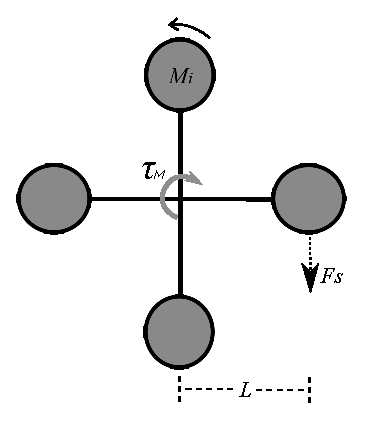
\includegraphics[width=6.5cm]{quadrotorTorque}    
		\caption{Motors torque experiment configuration} 
		\label{fig:quadrotortorque}
	\end{center}
\end{figure}
Taking into account that when the motor rotates clockwise, the quadrotor will tend to rotate counter-clockwise and vice versa, a scale is located to indirectly obtain the generated force $F_{s}$, using the reading of the weight $m_s$ as $F_{s} = m_{s}|\vec{g}|\ [N]$. Using (\ref{eqn:thrustvspwm}) and the \textit{PWM} width steps used in the motors thrust experiment, multiple $F_{M_i}$-dependent $F_s$ readings are obtained. The torques $\tau_M$ are then calculated by
\begin{equation}
\tau_{M} = F_{s}L\ [N\cdot m],
\end{equation}
and their results are shown in Fig. \ref{fig:torque_id}.
\begin{figure}[H]
	\begin{center}
		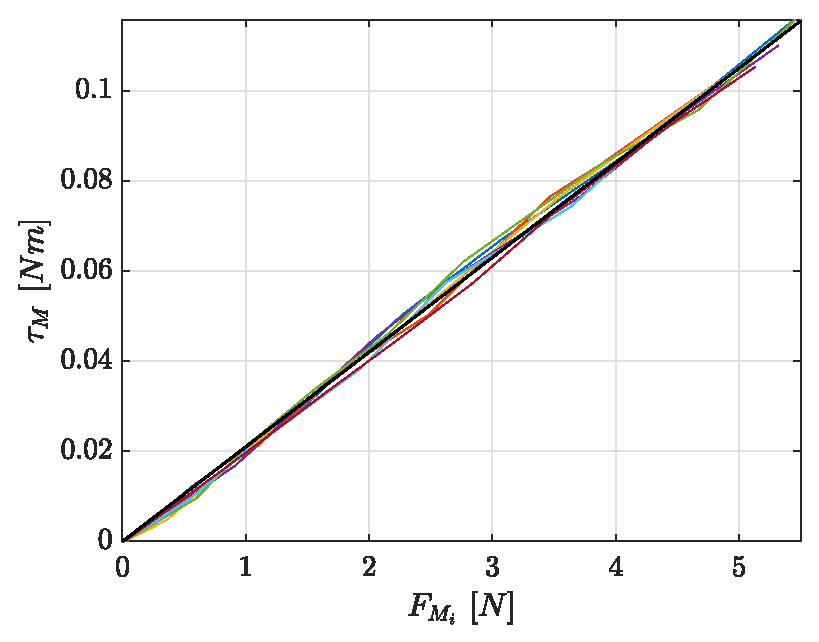
\includegraphics[width=9.5cm]{torque_id}    
		\caption{Torque} 
		\label{fig:torque_id}
	\end{center}
\end{figure}
The relation between $\tau_M$ and $F_{M_i}$ is linear as expected, and its slope defines the variable $K_m$ as
\begin{equation}
K_{m} = 0.021\ [m].
\end{equation}

\section{Conclusions}
This chapter presented the physical composition and parametrization of the smart- phone-based quadrotor prototype. In the first part, all the components of the quadrotor are detailed. A medium-size carbon fiber frame is used to support the complete quadrotor system. The LG Nexus 5X is selected as the smartphone where the control and estimation algorithms will be executed, which sends the control signals to an Arduino Mega ADK in order to generate \textit{PWM} signals that set the motors rotational velocities through the ESC. These components are supported and protected by 3D-printed objects that are attached to the carbon fiber frame. On the other hand, the system is parameterized in its entirety using experimental methods. Here, the total mass and moments of inertia of the system are defined using a scale and the bifilar pendulum experiment respectively, while the motor's thrust and torque about the $z$-axis are found applying multiple \textit{PWM} signals to the ESCs and obtaining the corresponding variable with the help of the scale.
\chapter{Control Strategies and State Estimation} \label{ch:controlandestimation}
This project seeks to evaluate control strategies designed for a quadrotor, test its performance in simulation, and then implement them in the smartphone-based quadrotor prototype. In this chapter, the design procedure of the control and estimation algorithms for the quadrotor is shown. This algorithms are based on the linearized model of the quadrotor, detailed in Section \ref{sec:linearized}. Also, all the simulations carried out in MATLAB to verify the proper functioning of the designed algorithms are exposed.
\\\\
The state-space representation of the system, and the concept of controllability and observability, are briefly introduced in Section \ref{sec:generalities}. Then, Section \ref{sec:controlstrategies} shows the theoretical basis required for the design of the controllers used in this project. This controllers are the Linear Quadratic Integral (LQI) controller and the $H_\infty$ controller.
\\\\
Section \ref{sec:controldesign} presents the considerations made for the design of the two types of controllers according to the flight mode of the quadrotor. In addition, this section shows the simulated response of the quadrotor being controlled by both types of controllers in each flight mode.
\\\\
Finally, the state estimation algorithm developed mainly for the case of the LQI controller, is detailed in Section \ref{sec:stateestimation}.

\section{Concept and Generalities}
\label{sec:generalities}

\subsection{State Space Representation}
Recalling from Section \ref{sec:linearized}, the dynamic model of the quadrotor, based on its six $DoF$, is represented by the linear state-space model
\begin{align}
\label{ec:statespace}
\begin{split}
\dot{\mathbf{x}}(t) & = A\mathbf{x}(t)+B\mathbf{u}(t),\\[10px]
\mathbf{y}(t) & = C\mathbf{x}(t)+D\mathbf{u}(t),
\end{split}
\end{align}
where $A$ is the system matrix; $B$ is the input matrix; $C$ is the output matrix; $D$ is the feed-through matrix; $\mathbf{x}$ is the states vector of size $\mathit{n_x}$; $\mathbf{u}$ is the inputs vector of size $\mathit{n_u}$; and $\mathbf{y}$ is the outputs vector of size $\mathit{n_y}$.
\\\\
For simplicity, the state-space model representation shown in (\ref{ec:statespace}), can be represented by the quartet of matrices $\mathcal{G}$ as
\begin{equation}\label{eqn:ss}
\mathcal{G} = \mleft[
\begin{array}{c|c}
  A & B \\
  \hline
  C & D
\end{array}
\mright].
\end{equation}
For the design of each controller, only the dynamics that are required to control, according to the flight mode in which the quadrotor is set, are taken into account. Therefore, system $\mathcal{G}$ will vary for each flight mode.

\subsection{Controllability and Observability}
The concept of controllability is related to the question of whether or not there exists a sequence of $\mathbf{u}$ capable of changing the states $\mathbf{x}$ from an initial value $\mathbf{x_0}$, to a desired final value $\mathbf{x_f}$, in a finite time. On the other hand, observability refers to the possibility of inferring, in finite time, the initial value of the states $\mathbf{x_0}$ knowing just the system dynamics $\mathcal{G}$ and its outputs $\mathbf{y}$ \cite{controlability1981}.
\\\\
Typically, the controllability and observability of a system are determined using the so-called controllability and observability matrices, $\mathcal{C_{G}}$ and $\mathcal{O_{G}}$ respectively.
This matrices depend on the system matrices $A$, $B$ and $C$, and are set as
\begin{align}
\begin{split}
\mathcal{C_{G}} & =
\begin{bmatrix}
B &  AB & \hdots & A^{k-1}B
\end{bmatrix},\\[5px]
\mathcal{O_G} & = \begin{bmatrix}
C\\
CA\\
\vdots\\
CA^{k-1}
\end{bmatrix}.
\end{split}
\end{align}
Thus, the system $\mathcal{G}$ is defined as controllable if $\mathcal{C_G}$ have $\mathit{n_x}$ linear independent rows (or columns). This is, the rank of $\mathcal{C_G}$ is equal to $\mathit{n_x}$. Analogous to the controllability, the observability of $\mathcal{G}$ is checked if the rank of the matrix $\mathcal{O_G}$ is equal to $\mathit{n_x}$.
\\\\
Another way to check the controllability and observability features of $\mathcal{G}$ is using the controllability and observability Grammians $\mathcal{W}_{c}$ and $\mathcal{W}_{o}$ defined as the solutions to the Lyapunov equations
\begin{align}
\begin{split}
0 & = A\mathcal{W}_{c} + \mathcal{W}_{c}A^{T} + BB^{T},\\[5px]
0 & = A^{T}\mathcal{W}_{o} + \mathcal{W}_{o}A + C^{T}C,
\end{split}
\end{align}
where
\begin{align}
\begin{split}
\mathcal{W}_{c} & = \int_{0}^{\infty}e^{At}BB^{T}e^{A^{T}t}dt,\\[5px]
\mathcal{W}_{o} & = \int_{0}^{\infty}e^{A^{T}t}C^{T}Ce^{At}dt.
\end{split}
\end{align}
In this case, if the matrices $\mathcal{W}_{c}$ and $\mathcal{W}_{o}$ are positive definite, the system is both controllable and observable \cite{Werner2012}.

\section{Control Strategies}
\label{sec:controlstrategies}
This section exposes the controllers design procedure. Here, the mathematical procedure to design a linear quadratic integral controller is described. It includes a regulator and an estimator, in addition to a gain compensator, allowing the system to track a trajectory. The design process of a $H_{\infty}$ controller is shown, taking into account some weighting sensitivities.

\subsection{Linear Quadratic Integral (LQI) Controller}
\subsubsection{Optimal Problem Solution}
The design of optimal controllers seeks that a dynamic system can be controlled achieving a minimum cost. The cost function is determined by the control designer \cite{Steinbuch2007}. Designing an finite-time regulator, a linear quadratic regulator (LQR) is set while looking for the minimization of the cost function $\mathcal{V}$ as
\begin{equation}
\mathcal{V} = \int_{0}^{T}\mathcal{L}(\mathbf{x},\mathbf{u},t)\ dt + \Psi(\mathbf{x},\mathbf{u},t),
\end{equation}
where
\begin{align}
\begin{split}
\mathcal{L}(\mathbf{x},\mathbf{u},t) = \mathbf{x}^{T}\mathcal{Q}\mathbf{x} + \mathbf{u}^{T}\mathcal{R}\mathbf{u},\\[5px]
\Psi(\mathbf{x},\mathbf{u},t) = \mathbf{x}^{T}(T)\mathcal{S}\mathbf{x}(T),
\end{split}
\end{align}
$\mathcal{R}$ is a positive definite matrix; and $\mathcal{Q}$ and $\mathcal{S}$ are positive semi-definite matrices. These matrices penalize the inputs, states and the terminal cost, respectively. Thus, the optimal controller design problem turns into an optimization problem where it is necessary to find an input $\mathbf{u}^{*}$ such that minimizes $\mathcal{V}$ for a controllable system subject to
\begin{align}
\begin{split}
\dot{\mathbf{x}}(t) & = \mathbf{f}(\mathbf{x}, \mathbf{u}, t) \approx A\mathbf{x}(t)+B\mathbf{u}(t),\\[5px]
\mathbf{x}(0) & = \mathbf{x_0},\ \ \ t \in [0, T].
\end{split}
\end{align}
This minimization is achieved using the Pontryagin's maximum principle \cite{Murray2009}, where
\begin{equation}
\mathcal{H}(\mathbf{x},\mathbf{u},\lambda_\mathcal{P},t) = \mathcal{L}(\mathbf{x},\mathbf{u},t) + \lambda_\mathcal{P}^{T}\mathbf{f}(\mathbf{x}, \mathbf{u}, t)
\end{equation}
is the Hamiltonian function, with $\lambda_\mathcal{P}$ being the vector of co-state variables of size $\mathit{n_x}$, and
\begin{align}
\label{eqn:hamilt}
\begin{split}
\dot{\mathbf{x}}(t) & = \left(\dfrac{\partial \mathcal{H}(\mathbf{x},\mathbf{u},\lambda_\mathcal{P},t)}{\partial \lambda_\mathcal{P}}\right)^{T} = A\mathbf{x}(t)+B\mathbf{u}(t),\\[5px]
-\dot{\lambda}_{\mathcal{P}}(t) & = \left(\dfrac{\partial \mathcal{H}(\mathbf{x},\mathbf{u},\lambda_\mathcal{P},t)}{\partial \mathbf{x}}\right)^{T} = \mathcal{Q}\mathbf{x}(t) + A^{T}\lambda_{\mathcal{P}}(t),\\[5px]
0 & = \dfrac{\partial \mathcal{H}(\mathbf{x},\mathbf{u},\lambda_\mathcal{P},t)}{\partial \mathbf{u}} = \mathcal{R}\mathbf{u}(t) + \lambda_\mathcal{P}^{T}(t)B.
\end{split}
\end{align}
Thereby, from (\ref{eqn:hamilt}), the optimal solution to $\mathbf{u}$ that minimizes $\mathcal{H}(\mathbf{x},\mathbf{u},\lambda_\mathcal{P},t)$, and by Pontryagin's maximum principle, the cost function $\mathcal{V}$, is
\begin{equation}
\mathbf{u}^{*}(t) = -\mathcal{R}^{-1}B^{T}\lambda_\mathcal{P}(t).
\end{equation}
Assuming that $\lambda_\mathcal{P}(t) = \mathcal{P}(t)\mathbf{x}(t)$, the optimal input $\mathbf{u}^{*}$ depends directly on a feedback vector, which is the state vector $\mathbf{x}$, such that
\begin{align}
\label{eqn:optimalu}
\begin{split}
\mathbf{u}^{*}(t) & = \mathbf{K_{lqr}}(t)\mathbf{x}(t),\\[5px]
\mathbf{K_{lqr}}(t) & = -\mathcal{R}^{-1}B^{T}\mathcal{P}(t).
\end{split}
\end{align}
Here, matrix $\mathcal{P}(t)$ is a solution of the Riccati Equation \cite{Moore1989}
	\begin{equation}
	-\dot{\mathcal{P}} = \mathcal{P}A + A^{T}\mathcal{P} + \mathcal{Q} - \mathcal{P}B\mathcal{R}^{-1}B^{T}\mathcal{P}.
	\end{equation}
When $T \to \infty$, an infinite-time regulator is designed. Here, aiming for a steady-state solution, the terminal cost $\Psi(\mathbf{x}, \mathbf{u},t)$ is eliminated, and the matrix $\mathcal{P}$ is assumed to be constant. Thus, $\mathcal{P}$ is a solution of the Algebraic Riccati Equation (ARE)
	\begin{equation}
	0 = \mathcal{P}A + A^{T}\mathcal{P} + \mathcal{Q} - \mathcal{P}B\mathcal{R}^{-1}B^{T}\mathcal{P}.
	\end{equation}
Consequently, in the infinite-time LQR, the optimal input $\mathbf{u}^{*}$ is achieved by multiplying the state vector $\mathbf{x}$ with the constant feedback gain matrix
\begin{equation}
\mathbf{K_{lqr}} = -\mathcal{R}^{-1}B^{T}\mathcal{P}.
\end{equation}
\\As the feedback gain is not a dynamical system, but a static matrix, the order of the closed-loop dynamics is the same as the one of the system dynamics $\mathcal{G}$. The closed-loop dynamics are written as
\begin{equation}
\dot{\mathbf{x}} = (A+B\mathbf{K_{lqr}})\mathbf{x}.
\end{equation}
When the desired state value $\mathbf{x_{des}}$ is different from zero, these reference value is applied to the dynamics through the feedback gain matrix as
\begin{equation}
\dot{\mathbf{x}} = (A+B\mathbf{K_{lqr}})\mathbf{x}-B\mathbf{K_{lqr}}\mathbf{x_{des}},
\end{equation}
due to the fact that the error $\mathbf{e} = \mathbf{x} - \mathbf{x_{des}}$ is used as the feedback vector of the LQR.

\subsubsection{Reference Tracking}
The LQR design is not made for reference tracking, but just for regulation. 
, to let the quadrotor track a defined trajectory, it is necessary to include a gain filter $v$ for the reference that compensates the total gain of the closed-loop system and enables the tracking of a reference input $r$. This gain filter is defined as
	\begin{equation}\label{eqn:v}
	v = -(C*(A+BF+F_{e}C)^{-1}*B)^{-1},
	\end{equation}
and its placing in the system is shown in Fig. \ref{fig:lqi}.
	\begin{figure}[h]
	\begin{center}
	\includegraphics[width=10.5cm]{lqi}
	\caption{Closed-loop system with gain compensation for the LQG controller aiming to track a reference.}
	\label{fig:lqi}
	\end{center}
	\end{figure}
\\where $G_{cl}$ is the closed-system with the LQG controller described in (\ref{eqn:ssgcl}).
\begin{equation}
\mathbf{x_i} = \int \mathbf{e}\ dt,\ \ \mathbf{x_i}(0) = \mathbf{0},
\end{equation}
\begin{equation}
\mathbf{x_{lqi}} = \begin{bmatrix}
\mathbf{x} \\
\mathbf{x_i}
\end{bmatrix},
\end{equation}
\begin{align}
\begin{split}
\begin{bmatrix}
\dot{\mathbf{x}}\\
\mathbf{\dot{x}_i}
\end{bmatrix} & = \begin{bmatrix}
A & \mathbf{0_{\mathit{n_y}\times \mathit{n_y}}} \\
-C & \mathbf{0_{\mathit{n_y}\times \mathit{n_y}}}
\end{bmatrix}\begin{bmatrix}
\mathbf{x} \\
\mathbf{x_i}
\end{bmatrix} + \begin{bmatrix}
B \\ \mathbf{0_{\mathit{n_y}\times \mathit{n_y}}}
\end{bmatrix}\mathbf{u} +  \begin{bmatrix}
\mathbf{0_{\mathit{n_x}\times \mathit{n_x}}} \\
\mathcal{I}_{\mathit{n_y}\times \mathit{n_y}}
\end{bmatrix}r \\[5px]
\mathbf{y} & = \begin{bmatrix}
C & \mathbf{0_{\mathit{n_y}\times \mathit{n_y}}}
\end{bmatrix}\begin{bmatrix}
\mathbf{x} \\
\mathbf{x_i}
\end{bmatrix}
\end{split}
\end{align}

\subsection{$H_\infty$ Controller}
\cite{Zhou1999}
For the design of the $H\infty$ controller, a generalized plant like the shown in the Fig. \ref{fig:augmentedPlant}, was built.
\begin{figure}[H]
	\begin{center}
	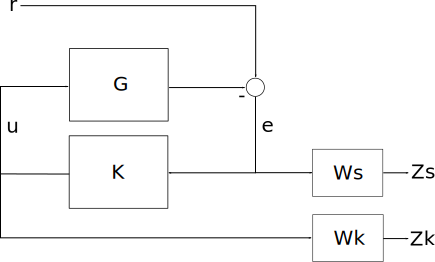
\includegraphics[width=6.5cm]{augmentedPlant.eps}
	\caption{Generalized plant with the weighting filters $W_s$ and $W_k$.}
	\label{fig:augmentedPlant}
	\end{center}
	\end{figure}	
In this generalized plant, $G$ represents the quadrotor dynamics, $K$ the controller, $r$ is the system reference, $e$ is the error, $u$ is the control input and $W_{s},\ W_{k}$ are weighting filters that must satisfy 
	\begin{equation}\label{eqn:hinf}
	\gamma = \left|\left|\begin{bmatrix}
	W_{s}S\\W_{k}KS
	\end{bmatrix}\right|\right|_{\infty} < 1,
	\end{equation}
\\where $S$ is the sensitivity function and $KS$ is the control sensitivity defined as
	\begin{equation}
	S = (\mathcal{I} + GK)^{-1},\ \ \ KS = K(\mathcal{I} + GK)^{-1}.
	\end{equation}
The weighting filters for the sensitivity and the control sensitivity were chosen as
\begin{align}\label{eqn:wswk}
\begin{split}
W_{S} &= \dfrac{w_{s}/M_{s}}{s + w_{s}}*\mathcal{I}_{4\times4}\ ,\\
W_{K} &= \dfrac{c}{M_{k}}\dfrac{s+w_{k}}{s+cw_{k}}*\mathcal{I}_{4\times4}\ ,
\end{split}
\end{align}
where $w_{s} = 10^{-4}$, $M_{s} = 10^{-4}$, $w_{k} = 20$, $M_{k} = 20$, and $c = 10^{3}$. With these weighting filters, the value of $\gamma$ is greater than one, and then it is necessary to rebuild the generalized plant using normalized weighting filters.
\\\\The $H_{\infty}$ controller can be simulated as shown in Fig. \ref{fig:hinfcontroller}.
	\begin{figure}[h]
	\begin{center}
	\includegraphics[width=7.0cm]{hinfcontroller.pdf}
	\caption{Closed-loop of the controlled system with an $H_{\infty}$ controller.}
	\label{fig:hinfcontroller}
	\end{center}
	\end{figure}
\subsubsection{$H_\infty$ Controller Order Reduction}
The designed $H_{\infty}$ controller for our quadrotor, will have 4 outputs (the quadrotor has 4 control inputs), 4 inputs (the quadrotor has 4 measured outputs) and 20 states (due to the 12 order plant, 4 order $W_{k}$ and 4 order $W_s$). To be able to implement this controller in a smartphone running Android, it it necessary to find a reduced order controller that behaves similarly to the full order controller $K$. To reduce the order of the controller, the singular values of the Hankel matrix
\begin{equation}
H_{k} = \begin{bmatrix}
C\\
CA\\
\vdots\\
CA^{k-1}
\end{bmatrix}
\begin{bmatrix}
B\\ AB \\ \vdots \\ A^{k-1}B
\end{bmatrix}^{T},
\end{equation}
are analysed. The energy of the Hankel singular values is shown in Fig. \ref{fig:hsv}.
\begin{figure}[h]
\begin{center}
\includegraphics[width=7.8cm]{HSV.pdf}  
\caption{Hankel singular values energy histogram of the designed controller.} 
\label{fig:hsv}
\end{center}
\end{figure}
\\\\As shown in Fig. \ref{fig:hsv}, the last ordered four states have unnoticeable energy when it is plotted; that means that these four states can be truncated from the controller without modifying its dynamics \cite{Skogestad2005}. 

\section{Controllers Design and Simulation}
\label{sec:controldesign}
fhfgfhfh
\subsection{Stabilize Mode}
fghgfh
\subsubsection{Dynamic Model}
\begin{align}
\begin{split}
\mathbf{x} = & \begin{bmatrix}
\psi & \dot{\psi} & \theta & \dot{\theta} & \phi & \dot{\phi}
\end{bmatrix}^{T},\\[15px]
\mathbf{y} = & \begin{bmatrix}
\psi & \theta & \phi
\end{bmatrix}^{T}
\end{split}
\end{align}
\begin{align}
\begin{split}
A = & 
\begin{bmatrix}
0 & 1 & 0 & 0 & 0 & 0 \\[2px]
0 & 0 & 0 & 0 & 0 & 0 \\[2px]
0 & 0 & 0 & 1 & 0 & 0 \\[2px]
0 & 0 & 0 & 0 & 0 & 0 \\[2px]
0 & 0 & 0 & 0 & 0 & 1 \\[2px]
0 & 0 & 0 & 0 & 0 & 0
\end{bmatrix}, \\[15px]
B = & 
\begin{bmatrix}
0 & 0 & 0 & 0 & 0 & 0\\[5px]
0 & \dfrac{1}{J_{zz}} & 0 & 0 & 0 & 0\\[5px]
0 & 0 & 0 & \dfrac{1}{J_{yy}} & 0 & 0\\[5px]
0 & 0 & 0 & 0 & 0 & \dfrac{1}{J_{xx}}
\end{bmatrix}^{T}.
\end{split}
\end{align}
\begin{align}
\begin{split}
C = & 
\begin{bmatrix}
1 & 0 & 0 & 0 & 0 & 0 \\[2px]
0 & 0 & 1 & 0 & 0 & 0 \\[2px]
0 & 0 & 0 & 0 & 1 & 0
\end{bmatrix}, \\[15px]
D = &\ \mathbf{0_{3\times 4}}.
\end{split}
\end{align}
\subsubsection{Linear Quadratic Regulator}
rtrte

\begin{figure}[H]
\begin{subfigure}{.5\linewidth}
\centering
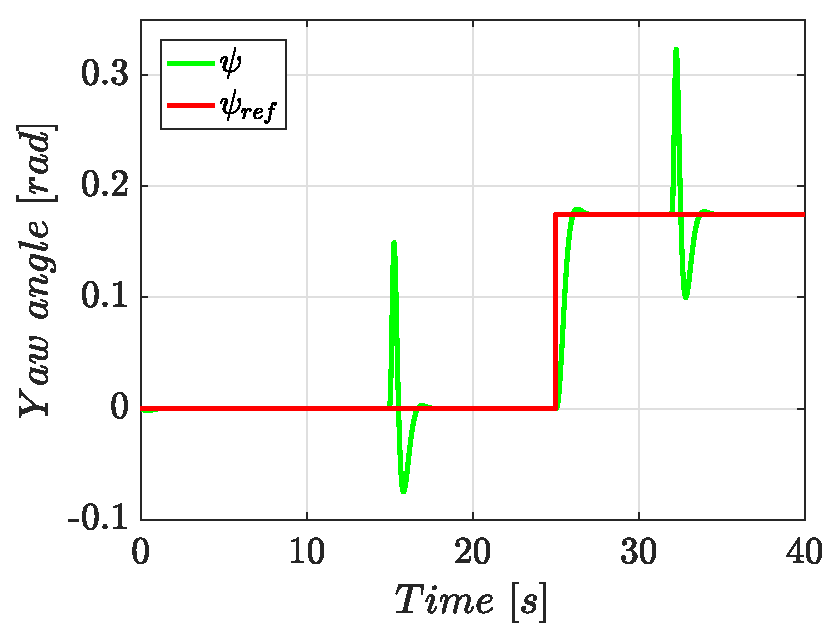
\includegraphics[width=7.0cm]{stabilize_psi_lqi}
\caption{Rotation about $x$ axis, $J_{xx}$ experiment}
\label{fig:stabilize_psi_lqi}
\end{subfigure}%
\begin{subfigure}{.5\linewidth}
\centering
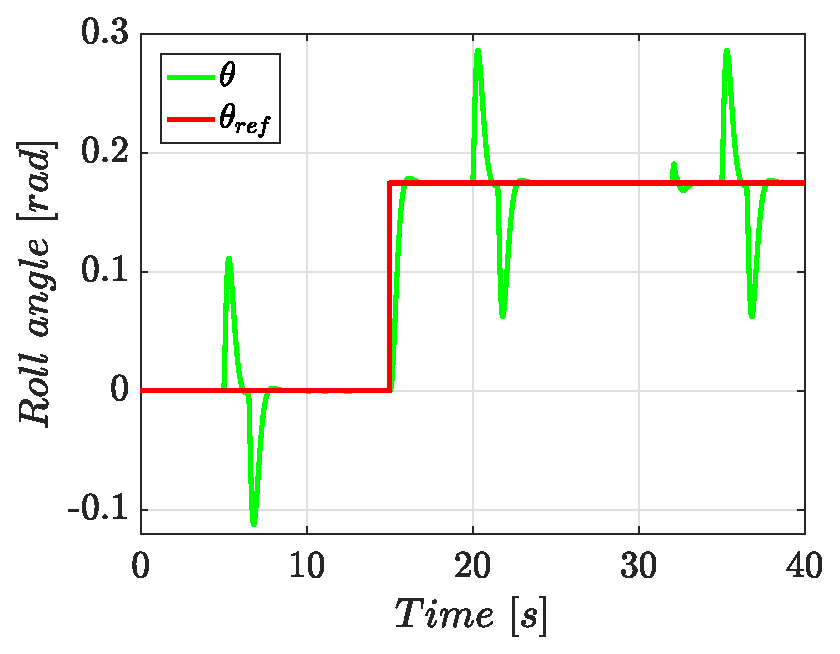
\includegraphics[width=7.0cm]{stabilize_theta_lqi}
\caption{Rotation about $y$ axis, $J_{yy}$ experiment}
\label{fig:stabilize_theta_lqi}
\end{subfigure}\\[1ex]
\begin{subfigure}{\linewidth}
\centering
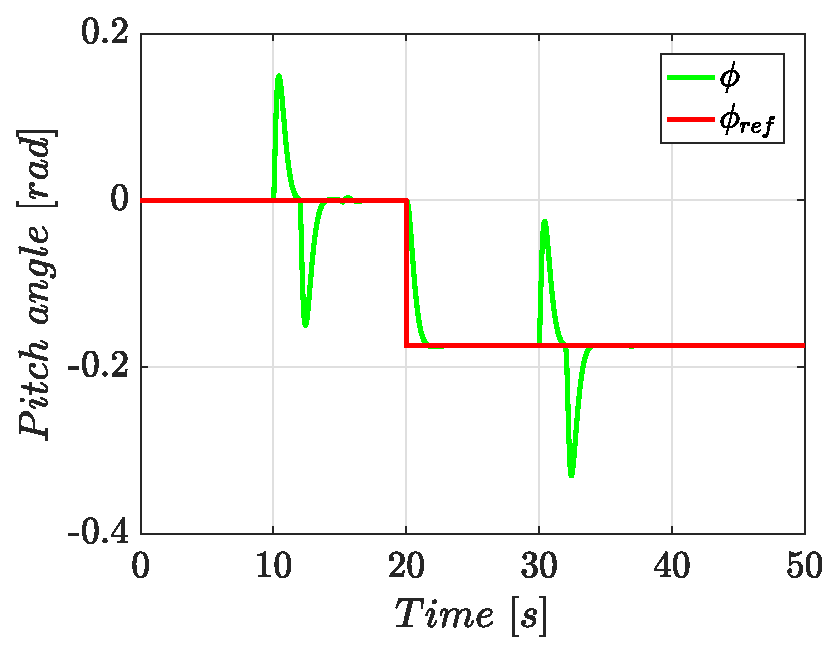
\includegraphics[width=7.0cm]{stabilize_phi_lqi}
\caption{Rotation about $z$ axis, $J_{zz}$ experiment}
\label{fig:stabilize_psi_lqi}
\end{subfigure}
\caption{Rotation about $x$, $y$ and $z$ axes during the bifilar pendulum experiments}
\label{fig:stabilize_lqi}
\end{figure}

\subsubsection{$H_\infty$ Controller}
rtrtererre
\begin{figure}[H]
\begin{subfigure}{.5\linewidth}
\centering
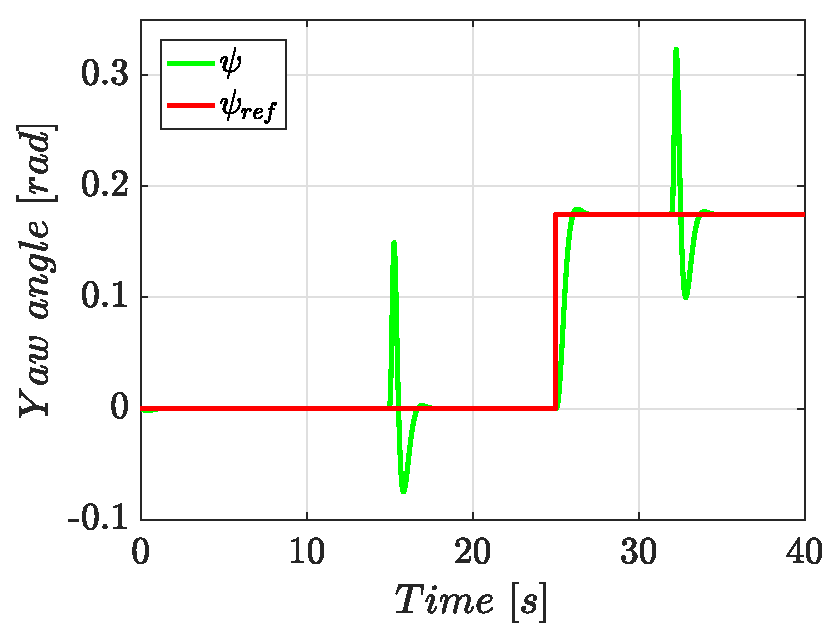
\includegraphics[width=7.0cm]{stabilize_psi_lqi}
\caption{Rotation about $x$ axis, $J_{xx}$ experiment}
\label{fig:stabilize_psi_lqi}
\end{subfigure}%
\begin{subfigure}{.5\linewidth}
\centering
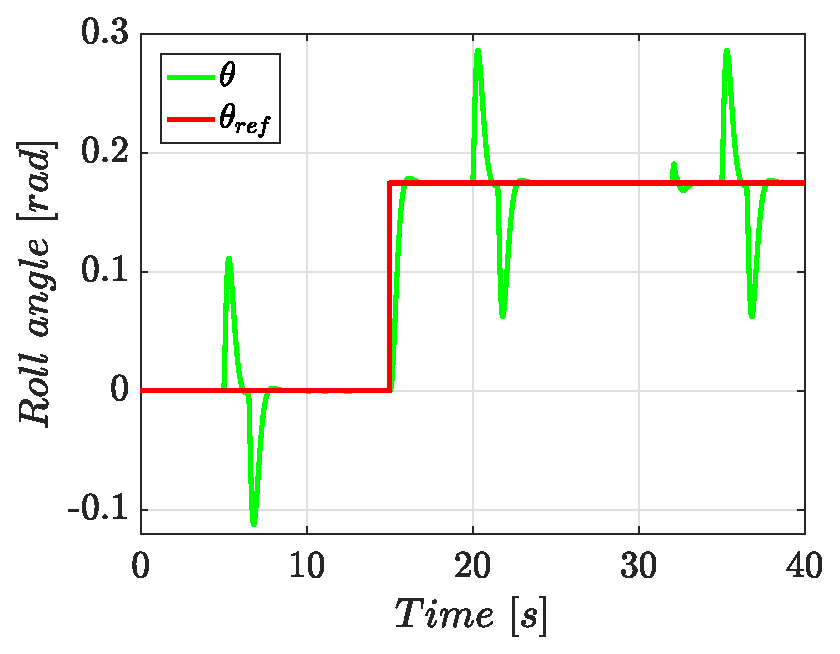
\includegraphics[width=7.0cm]{stabilize_theta_lqi}
\caption{Rotation about $y$ axis, $J_{yy}$ experiment}
\label{fig:stabilize_theta_lqi}
\end{subfigure}\\[1ex]
\begin{subfigure}{\linewidth}
\centering
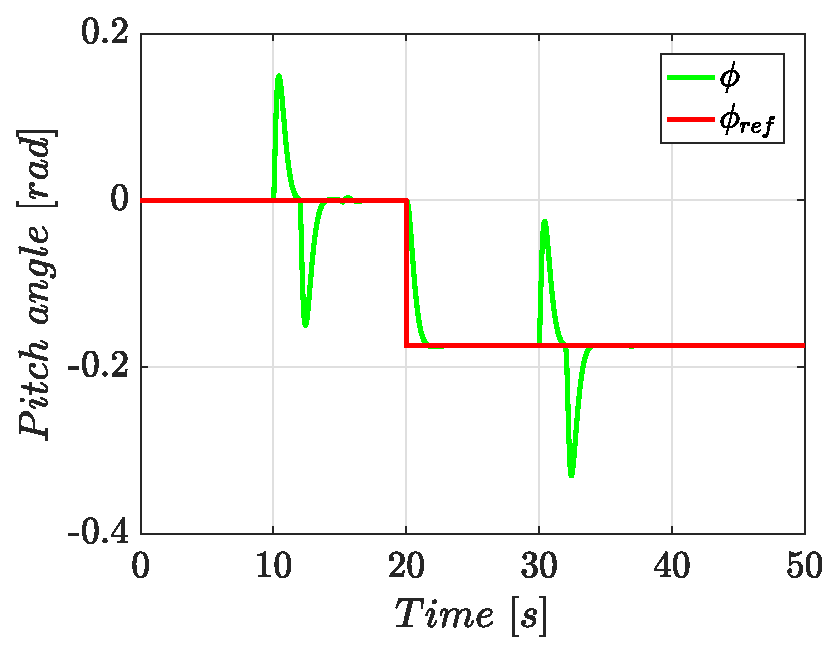
\includegraphics[width=7.0cm]{stabilize_phi_lqi}
\caption{Rotation about $z$ axis, $J_{zz}$ experiment}
\label{fig:stabilize_psi_lqi}
\end{subfigure}
\caption{Rotation about $x$, $y$ and $z$ axes during the bifilar pendulum experiments}
\label{fig:stabilize_lqi}
\end{figure}


\subsection{Altitude Hold Mode}
\subsubsection{Dynamic Model}

\begin{align}
\begin{split}
\mathbf{x} = & \begin{bmatrix}
z & \dot{z} & \psi & \dot{\psi} & \theta & \dot{\theta} & \phi & \dot{\phi}
\end{bmatrix}^{T},\\[15px]
\mathbf{y} = & \begin{bmatrix}
z & \psi & \theta & \phi
\end{bmatrix}^{T}
\end{split}
\end{align}
\begin{align}
\begin{split}
A = & 
\begin{bmatrix}
0 & 1 & 0 & 0 & 0 & 0 & 0 & 0\\[2px]
0 & 0 & 0 & 0 & 0 & 0 & 0 & 0\\[2px]
0 & 0 & 0 & 1 & 0 & 0 & 0 & 0\\[2px]
0 & 0 & 0 & 0 & 0 & 0 & 0 & 0\\[2px]
0 & 0 & 0 & 0 & 0 & 1 & 0 & 0\\[2px]
0 & 0 & 0 & 0 & 0 & 0 & 0 & 0\\[2px]
0 & 0 & 0 & 0 & 0 & 0 & 0 & 1\\[2px]
0 & 0 & 0 & 0 & 0 & 0 & 0 & 0
\end{bmatrix}, \\[15px]
B = & 
\begin{bmatrix}
0 & \dfrac{1}{m} & 0 & 0 & 0 & 0 & 0 & 0\\[5px]
0 & 0 & 0 & \dfrac{1}{J_{zz}} & 0 & 0 & 0 & 0\\[5px]
0 & 0 & 0 & 0 & 0 & \dfrac{1}{J_{yy}} & 0 & 0\\[5px]
0 & 0 & 0 & 0 & 0 & 0 & 0 & \dfrac{1}{J_{xx}}
\end{bmatrix}^{T}.
\end{split}
\end{align}
\begin{align}
\begin{split}
C = & 
\begin{bmatrix}
1 & 0 & 0 & 0 & 0 & 0 & 0 & 0 \\[2px]
0 & 0 & 1 & 0 & 0 & 0 & 0 & 0 \\[2px]
0 & 0 & 0 & 0 & 1 & 0 & 0 & 0 \\[2px]
0 & 0 & 0 & 0 & 0 & 0 & 1 & 0 
\end{bmatrix}, \\[15px]
D = &\ \mathbf{0_{4\times 4}}.
\end{split}
\end{align}
\subsubsection{Linear Quadratic Regulator}
rtrterere
\begin{figure}[H]
\begin{subfigure}{.5\linewidth}
\centering
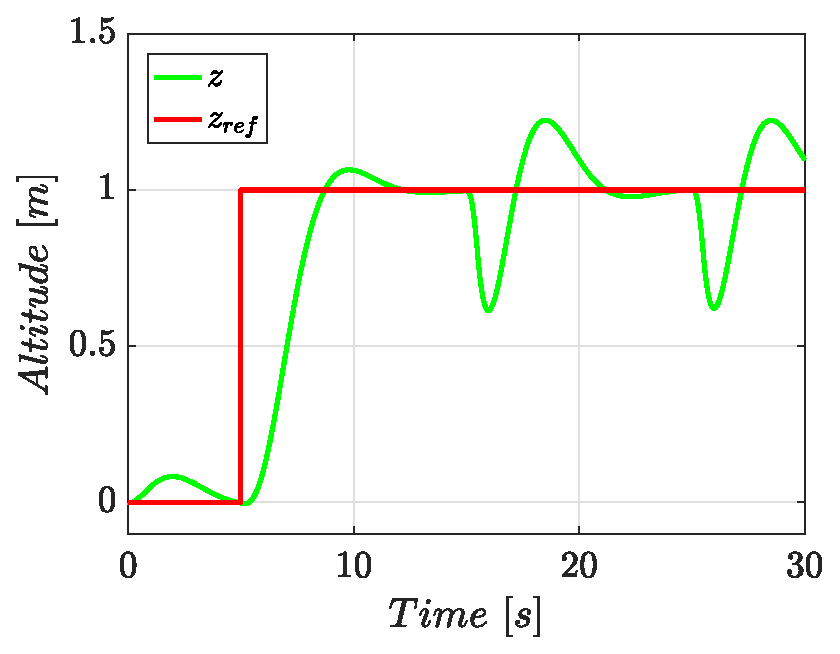
\includegraphics[width=7.0cm]{althold_z_lqi}
\caption{Rotation about $x$ axis, $J_{xx}$ experiment}
\label{fig:althold_z_lqi}
\end{subfigure}%
\begin{subfigure}{.5\linewidth}
\centering
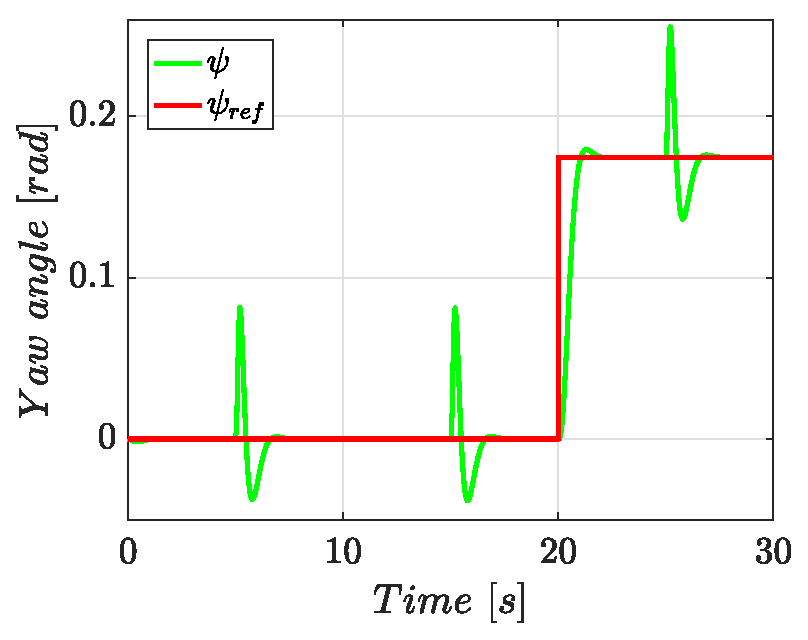
\includegraphics[width=7.0cm]{althold_psi_lqi}
\caption{Rotation about $y$ axis, $J_{yy}$ experiment}
\label{fig:althold_psi_lqi}
\end{subfigure}\\[1ex]
\begin{subfigure}{0.5\linewidth}
\centering
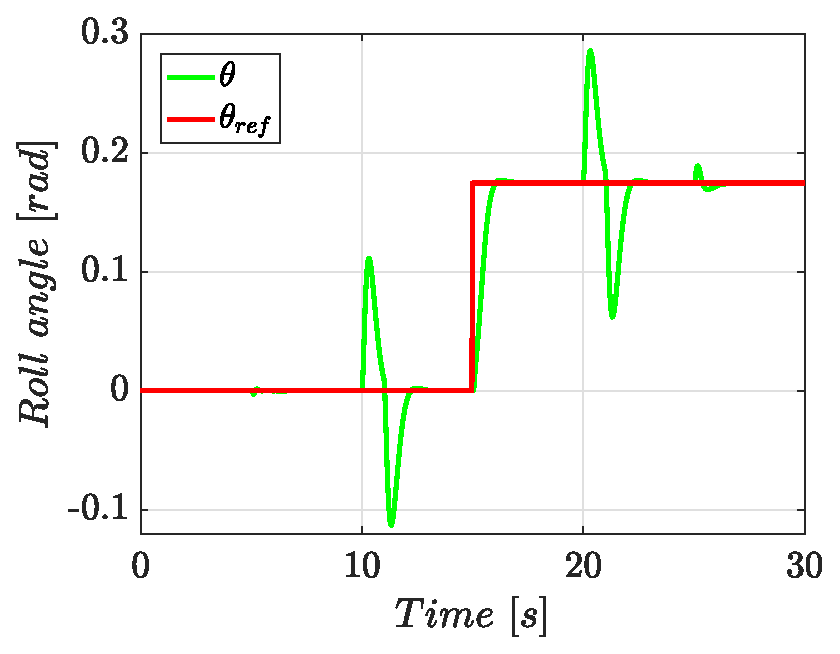
\includegraphics[width=7.0cm]{althold_theta_lqi}
\caption{Rotation about $z$ axis, $J_{zz}$ experiment}
\label{fig:althold_theta_lqi}
\end{subfigure}
\begin{subfigure}{0.5\linewidth}
\centering
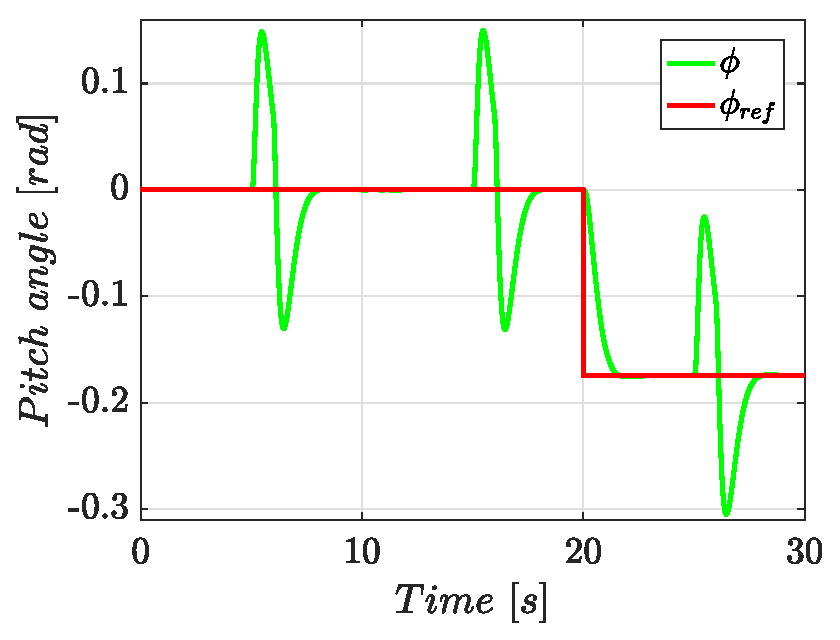
\includegraphics[width=7.0cm]{althold_phi_lqi}
\caption{Rotation about $z$ axis, $J_{zz}$ experiment}
\label{fig:althold_phi_lqi}
\end{subfigure}
\caption{Rotation about $x$, $y$ and $z$ axes during the bifilar pendulum experiments}
\label{fig:althold_lqi}
\end{figure}

\subsubsection{$H_\infty$ Controller}
rtrtererre

\begin{figure}[H]
\begin{subfigure}{.5\linewidth}
\centering
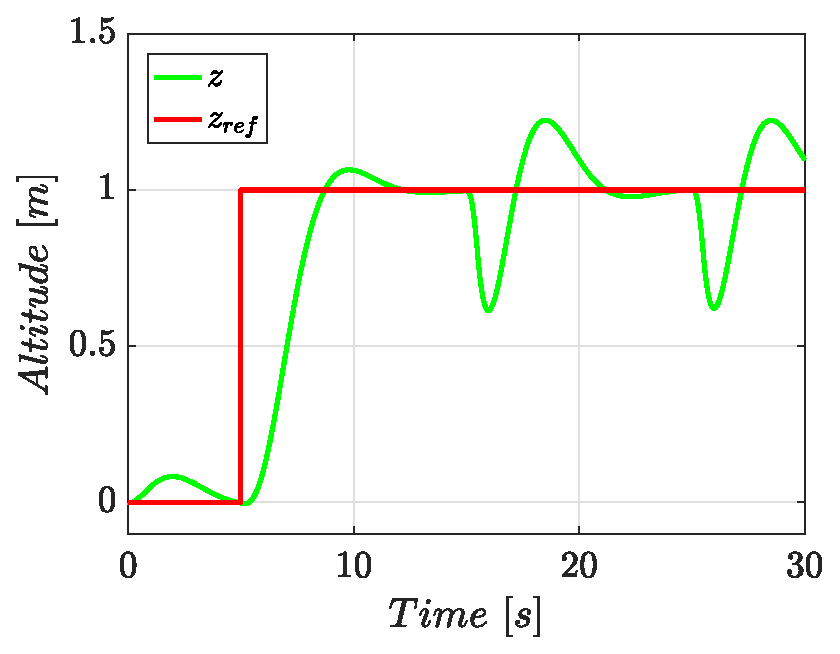
\includegraphics[width=7.0cm]{althold_z_lqi}
\caption{Rotation about $x$ axis, $J_{xx}$ experiment}
\label{fig:althold_z_lqi}
\end{subfigure}%
\begin{subfigure}{.5\linewidth}
\centering
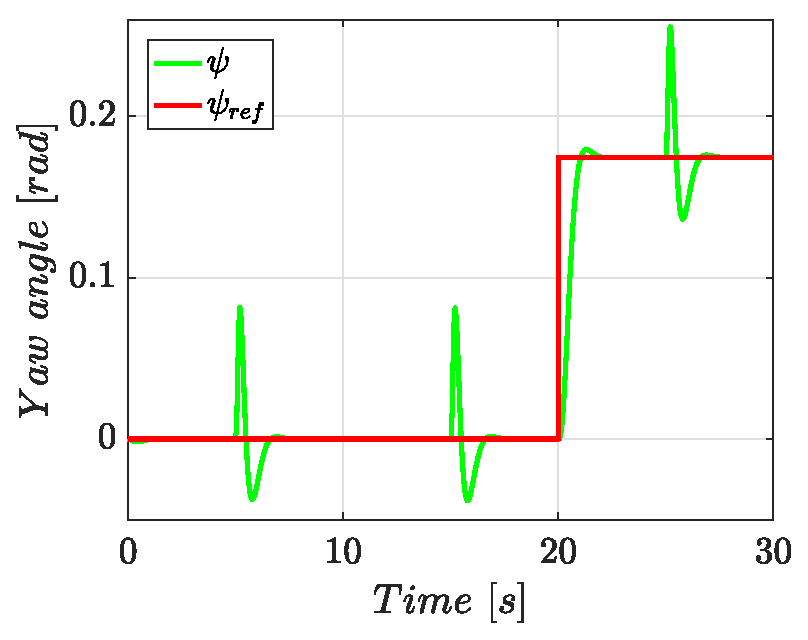
\includegraphics[width=7.0cm]{althold_psi_lqi}
\caption{Rotation about $y$ axis, $J_{yy}$ experiment}
\label{fig:althold_psi_lqi}
\end{subfigure}\\[1ex]
\begin{subfigure}{0.5\linewidth}
\centering
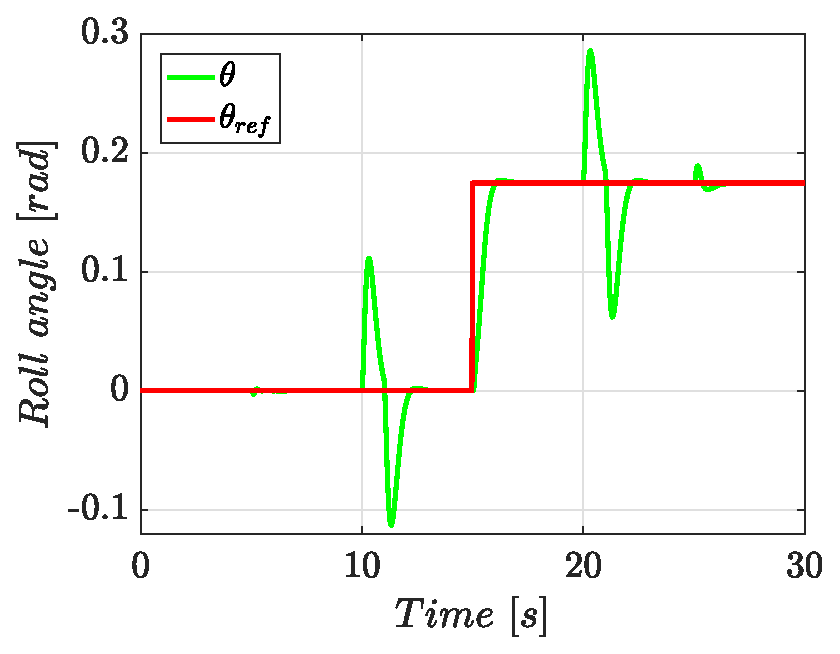
\includegraphics[width=7.0cm]{althold_theta_lqi}
\caption{Rotation about $z$ axis, $J_{zz}$ experiment}
\label{fig:althold_theta_lqi}
\end{subfigure}
\begin{subfigure}{0.5\linewidth}
\centering
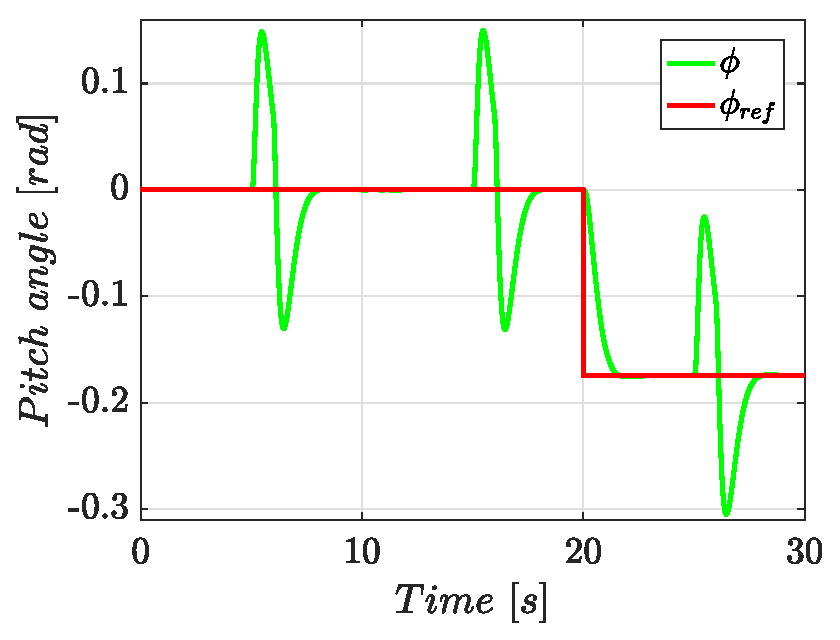
\includegraphics[width=7.0cm]{althold_phi_lqi}
\caption{Rotation about $z$ axis, $J_{zz}$ experiment}
\label{fig:althold_phi_lqi}
\end{subfigure}
\caption{Rotation about $x$, $y$ and $z$ axes during the bifilar pendulum experiments}
\label{fig:althold_lqi}
\end{figure}

\subsection{GNSS Dependent Flight Modes}

\subsubsection{Dynamic Model}
\begin{align}
\begin{split}
\mathbf{x} = & \begin{bmatrix}
x & \dot{x} & y & \dot{y} & z & \dot{z} & \psi & \dot{\psi} & \theta & \dot{\theta} & \phi & \dot{\phi}
\end{bmatrix}^{T},\\[15px]
\mathbf{y} = & \begin{bmatrix}
x & y & z & \psi & \theta & \phi
\end{bmatrix}^{T}
\end{split}
\end{align}

\begin{align}
\begin{split}
A = & 
\begin{bmatrix}
0 & 1 & 0 & 0 & 0 & 0 & 0 & 0 & 0 & 0 & 0 & 0\\[2px]
0 & 0 & 0 & 0 & 0 & 0 & 0 & 0 & g & 0 & 0 & 0\\[2px]
0 & 0 & 0 & 1 & 0 & 0 & 0 & 0 & 0 & 0 & 0 & 0\\[2px]
0 & 0 & 0 & 0 & 0 & 0 & 0 & 0 & 0 & 0 & g & 0\\[2px]
0 & 0 & 0 & 0 & 0 & 1 & 0 & 0 & 0 & 0 & 0 & 0\\[2px]
0 & 0 & 0 & 0 & 0 & 0 & 0 & 0 & 0 & 0 & 0 & 0\\[2px]
0 & 0 & 0 & 0 & 0 & 0 & 0 & 1 & 0 & 0 & 0 & 0\\[2px]
0 & 0 & 0 & 0 & 0 & 0 & 0 & 0 & 0 & 0 & 0 & 0\\[2px]
0 & 0 & 0 & 0 & 0 & 0 & 0 & 0 & 0 & 1 & 0 & 0\\[2px]
0 & 0 & 0 & 0 & 0 & 0 & 0 & 0 & 0 & 0 & 0 & 0\\[2px]
0 & 0 & 0 & 0 & 0 & 0 & 0 & 0 & 0 & 0 & 0 & 1\\[2px]
0 & 0 & 0 & 0 & 0 & 0 & 0 & 0 & 0 & 0 & 0 & 0
\end{bmatrix}, \\[15px]
B = & 
\begin{bmatrix}
0 & 0 & 0 & 0 & 0 & \dfrac{1}{m} & 0 & 0 & 0 & 0 & 0 & 0\\[5px]
0 & 0 & 0 & 0 & 0 & 0 & 0 & \dfrac{1}{J_{zz}} & 0 & 0 & 0 & 0\\[5px]
0 & 0 & 0 & 0 & 0 & 0 & 0 & 0 & 0 & \dfrac{1}{J_{yy}} & 0 & 0\\[5px]
0 & 0 & 0 & 0 & 0 & 0 & 0 & 0 & 0 & 0 & 0 & \dfrac{1}{J_{xx}}
\end{bmatrix}^{T}.
\end{split}
\end{align}
\begin{align}
\begin{split}
C = & 
\begin{bmatrix}
1 & 0 & 0 & 0 & 0 & 0 & 0 & 0 & 0 & 0 & 0 & 0 \\[2px]
0 & 0 & 1 & 0 & 0 & 0 & 0 & 0 & 0 & 0 & 0 & 0 \\[2px]
0 & 0 & 0 & 0 & 1 & 0 & 0 & 0 & 0 & 0 & 0 & 0 \\[2px]
0 & 0 & 0 & 0 & 0 & 0 & 1 & 0 & 0 & 0 & 0 & 0 \\[2px]
0 & 0 & 0 & 0 & 0 & 0 & 0 & 0 & 1 & 0 & 0 & 0 \\[2px]
0 & 0 & 0 & 0 & 0 & 0 & 0 & 0 & 0 & 0 & 1 & 0
\end{bmatrix}, \\[15px]
D = &\ \mathbf{0_{6\times 4}}.
\end{split}
\end{align}
\subsubsection{Linear Quadratic Regulator}
rtrterere
\begin{figure}[h]
	\begin{center}
	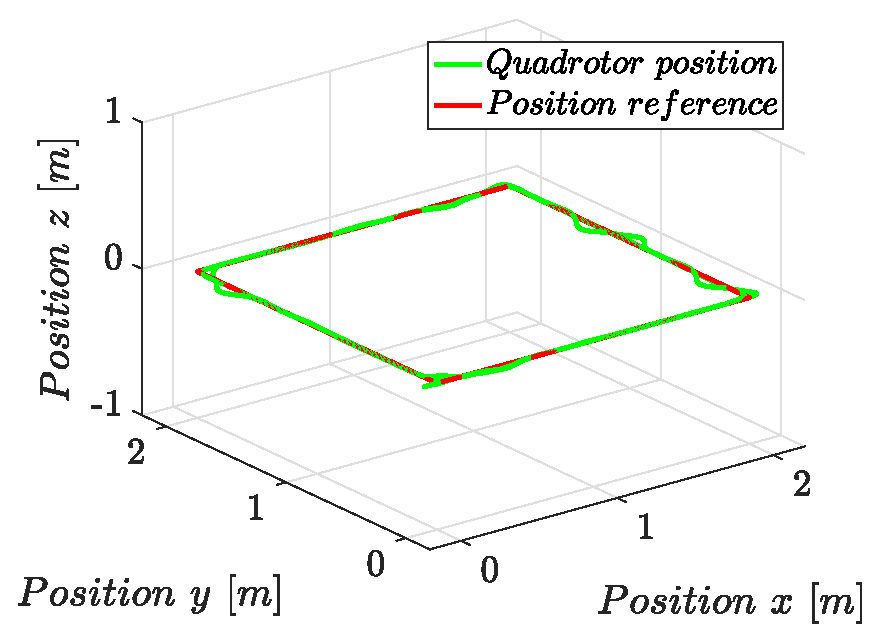
\includegraphics[width=0.8\textwidth]{auto_xyz_lqi}
	\caption{Closed-loop of the controlled system with an $H_{\infty}$ controller.}
	\label{fig:auto_xyz_lqi}
	\end{center}
	\end{figure}
	
\begin{figure}[H]
\begin{subfigure}{.5\linewidth}
\centering
\includegraphics[width=7.0cm]{auto_psi_lqi}
\caption{Rotation about $x$ axis, $J_{xx}$ experiment}
\label{fig:auto_psi_lqi}
\end{subfigure}%
\begin{subfigure}{.5\linewidth}
\centering
\includegraphics[width=7.0cm]{auto_theta_lqi}
\caption{Rotation about $y$ axis, $J_{yy}$ experiment}
\label{fig:auto_theta_lqi}
\end{subfigure}\\[1ex]
\begin{subfigure}{\linewidth}
\centering
\includegraphics[width=7.0cm]{auto_phi_lqi}
\caption{Rotation about $z$ axis, $J_{zz}$ experiment}
\label{fig:auto_psi_lqi}
\end{subfigure}
\caption{Rotation about $x$, $y$ and $z$ axes during the bifilar pendulum experiments}
\label{fig:auto_lqi}
\end{figure}

\subsubsection{$H_\infty$ Controller}
rtrtererre

\begin{figure}[h]
	\begin{center}
	\includegraphics[width=0.8\textwidth]{auto_xyz_lqi}
	\caption{Closed-loop of the controlled system with an $H_{\infty}$ controller.}
	\label{fig:auto_xyz_lqi}
	\end{center}
	\end{figure}
	
\begin{figure}[H]
\begin{subfigure}{.5\linewidth}
\centering
\includegraphics[width=7.0cm]{auto_psi_lqi}
\caption{Rotation about $x$ axis, $J_{xx}$ experiment}
\label{fig:auto_psi_lqi}
\end{subfigure}%
\begin{subfigure}{.5\linewidth}
\centering
\includegraphics[width=7.0cm]{auto_theta_lqi}
\caption{Rotation about $y$ axis, $J_{yy}$ experiment}
\label{fig:auto_theta_lqi}
\end{subfigure}\\[1ex]
\begin{subfigure}{\linewidth}
\centering
\includegraphics[width=7.0cm]{auto_phi_lqi}
\caption{Rotation about $z$ axis, $J_{zz}$ experiment}
\label{fig:auto_psi_lqi}
\end{subfigure}
\caption{Rotation about $x$, $y$ and $z$ axes during the bifilar pendulum experiments}
\label{fig:auto_lqi}
\end{figure}

\section{State Estimation Through Kalman Filter}
\label{sec:stateestimation}
The quadrotor dynamics are sensed exclusively using the on-board smartphone's sensors. Considering that these sensors have different sample frequencies, and poor accuracy, it is necessary to use estimation algorithms, as a Kalman filter, to get reliable state data with constant sample frequency.

\subsection{Attitude Estimation}
The Android API implements a Kalman filter for attitude estimation using the raw data deliverd by the smartphone's accelerometer, gyroscope and magnetometer, as exposed in \cite{Astudillo2017}. Using the quaternion $Q_s$ delivered by the Rotation virtual sensor included in the Android SDK, it is obtained an absolute orientation representation with respect to the Earth frame \cite{AndSensor}, with
\begin{align}\label{eqn:rotvector}
\begin{split}
Q_{s} &= \mathrm{e}^{(\alpha/2)(u\vv{i}+v\vv{j}+w\vv{k})} \\
&= \begin{bmatrix}
u\sin(\alpha / 2)\\
v\sin(\alpha / 2)\\
w\sin(\alpha / 2)\\
\cos(\alpha / 2)
\end{bmatrix} = \begin{bmatrix}
q_{0} \\
q_{1} \\
q_{2} \\
q_{3}
\end{bmatrix}
\end{split}
\end{align}
where $\alpha$ is the amount of degrees the quaternion is rotated around the axis $u\vv{i}+v\vv{j}+w\vv{k}$. The rotation matrix $R_{b}^{w}$ can be defined using $Q_s$ as
\begin{equation}
R_{b}^{w} = \begin{bmatrix}
1-2(q_{2}^{2}+q_{3}^{2}) & 2(q_{1}q_{2}-q_{0}q_{3}) & 2(q_{0}q_{2}+q_{1}q_{3}) \\
2(q_{1}q_{2}-q_{0}q_{3}) & 1-2(q_{1}^{2}+q_{3}^{2}) & 2(q_{2}q_{3}+q_{0}q_{1}) \\
2(q_{1}q_{3}+q_{0}q_{2}) & 2(q_{0}q_{1}+q_{2}q_{3}) & 1-2(q_{1}^{2}+q_{2}^{2})
\end{bmatrix}.
\end{equation}
Comparing the terms in the two representations of $R_{b}^{w}$, the Euler angles are obtained as
\begin{equation}\label{eqn:quattoeu}
\begin{bmatrix}
\psi \\
\theta \\
\phi
\end{bmatrix} =
\begin{bmatrix}
atan2(2(q_{3}q_{2} + q_{0}q{1}),1-2(q_{1}^{2} + q_{2}^{2})) \\
arcsin(2(q_{3}q_{1} - q_{2}q_{0})) \\
atan2(2(q_{3}q_{0} + q_{1}q{2}),1-2(q_{0}^{2} + q_{1}^{2})) 
\end{bmatrix}.
\end{equation}

\subsection{Position Estimation}
Taking into account that the global navigation satellite systems (GNSS) receivers in smartphones have an accuracy of around $3\ m$ and a sampling frequency of $1\ Hz$, a Kalman filter for position tracking is designed. In order to keep the estimation system independent from the application of controlling the quadrotor, this filter is based on the dynamics of a moving particle with constant acceleration between two samples
\begin{equation}
\xi(k+1) = \xi(k) + \dot{\xi}(k)t_{k} + 0.5\ddot{\xi}(k)t_{k}^{2},
\end{equation}
where $t_{k}$ is the sample time.\\\\
Using $E_{k} = \begin{bmatrix}
\xi & \dot{\xi} & \ddot{\xi}
\end{bmatrix}^{T}
 =
\begin{bmatrix}x_{k} & y_{k} & z_{k} & \dot{x}_{k} & \dot{y}_{k} & \dot{z}_{k} & \ddot{x}_{k} & \ddot{y}_{k} & \ddot{z}_{k} \end{bmatrix}^{T}$ as state vector and being 
\begin{equation}\label{eqn:A}
\Gamma = \begin{bmatrix}
   				 1 & 0 & 0 & t_{k} & 0 & 0 & 0.5t_{k}^{2} & 0 & 0\\
   				 0 & 1 & 0 & 0 & t_{k} & 0 & 0 & 0.5t_{k}^{2} & 0\\
   				 0 & 0 & 1 & 0 & 0 & t_{k} & 0 & 0 & t_{k}^{2}\\
   				 0 & 0 & 0 & 1 & 0 & 0 & t_{k} & 0 & 0\\
   				 0 & 0 & 0 & 0 & 1 & 0 & 0 & t_{k} & 0 \\
   				 0 & 0 & 0 & 0 & 0 & 1 & 0 & 0 & t_{k} \\
   				 0 & 0 & 0 & 0 & 0 & 0 & 1 & 0 & 0\\
   				 0 & 0 & 0 & 0 & 0 & 0 & 0 & 1 & 0\\
   				 0 & 0 & 0 & 0 & 0 & 0 & 0 & 0 & 1 
				\end{bmatrix},
\end{equation}
the matrix that satisfies $E_{k+1} = \Gamma E_{k}$, the prediction of the state $\hat{E}_{k}^{-}$ and its covariance $P_{k}^{-}$ are obtained as
\begin{equation}\label{eqn:statePrognosis}
\hat{E}_{k}^{-} = \Gamma \hat{E}_{k-1},
\end{equation}
\begin{equation}\label{eqn:covariancePrognosis}
P_{k}^{-} = \Gamma P_{k-1} \Gamma^{T} + Q_{k},
\end{equation}
where $\hat{E}_{k-1}$ is the previous estimated state, $P_{k-1}$ the previous error covariance matrix and $Q_{k}$ the process variance. The state prediction is then corrected calculating the Kalman gain vector $K_k$ as
\begin{align}\label{eqn:correctionKalman}
\begin{split}
K_{k} &= P^{-}_{k}H^{T}(HP^{-}_{k}H^{T} + R)^{-1},
\end{split}
\end{align}
and updating the state estimation $\hat{E}_{k}$ and its covariance $P_{k}$, based on the measurements $\zeta_k$ as
\begin{align}\label{eqn:correctionKalman2}
\begin{split}
\hat{E}_{k} &= \hat{E}^{-}_{k} + K_{k}(\zeta_{k} - H\hat{E}^{-}_{k}),\\
P_{k} &= (\mathcal{I} - K_{k}H)P^{-}_{k},
\end{split}
\end{align}
where $R$ is the measurement covariance matrix, $\mathcal{I}$ is the identity matrix and $H$ is the matrix that relate $\zeta_k$ and $E_k$. $H$ is defined as
\begin{equation}\label{eqn:H}
H =\begin{bmatrix}
			1 & 0 & 0 & 0 & 0 & 0 & 0 & 0 & 0\\
			0 & 1 & 0 & 0 & 0 & 0 & 0 & 0 & 0\\
			0 & 0 & 1 & 0 & 0 & 0 & 0 & 0 & 0\\
			0 & 0 & 0 & 0 & 0 & 0 & 1 & 0 & 0\\
			0 & 0 & 0 & 0 & 0 & 0 & 0 & 1 & 0\\
			0 & 0 & 0 & 0 & 0 & 0 & 0 & 0 & 1
			\end{bmatrix},
\end{equation}
considering that $\zeta_k \in R^{6}$ contains the GNSS measurements of $x_{m}$ and $y_{m}$, the barometer measurements of $z_{m}$ (in $m$), and the measurements of $\ddot{x}_{m}$, $\ddot{y}_{m}$ and $\ddot{z}_{m}$ in the Earth frame (in $m/s^{2}$).
\\\\
The $x_{m}$ and $y_{m}$ position measurements are acquired using the GNSS receiver in the smartphone. Each sample of these coordinates are initially set in an ellipsoidal representation of decimal degrees by the receiver, and then converted to a bi-dimensional representation in meter units using the cartographic projection Magna-Sirgas.
\\
The $z_{m}$ measurements are acquired using the barometric pressure sensor which delivers the pressure value $p_k$ in hPa. This signal is converted to meters as
\begin{equation}\label{eqn:hbarom}
z_{m} = 44330\left(1-\frac{p_k}{p_{0}}^{1/5.255}\right),
\end{equation}
where $p_{0}$ is the atmospheric pressure at sea level \cite{Lauszus2015}.\\\\
The remaining measurement signals are the accelerations with respect to the Earth frame, $\ddot{\xi}_{m}$. These signals are calculated using the raw acceleration measurements from the smartphone $a_{b}$, which are represented with respect to the smartphone's body frame, and the attitude quaternion $Q_s$ as
\begin{equation}
\ddot{\xi}_{m} = \begin{bmatrix}
\ddot{x}_{m} & \ddot{y}_{m} & \ddot{z}_{m}
\end{bmatrix}^{T} =Q_{s}a_{b}Q'_{s},
\end{equation}
where $Q'_{s}$ is the quaternion conjugate of $Q_{s}$.
\\\\
The vector $\zeta_k$ is then set as
\begin{equation}
\zeta_k = \begin{bmatrix}
x_{m} & y_{m} & z_{m} & \ddot{x}_{m} & \ddot{y}_{m} & \ddot{z}_{m}
\end{bmatrix}^{T}.
\end{equation}

\subsection{Particle Model}
rtrtrtrtrt

\subsection{Quadrotor Model}
ytytyttytt

\section{Conclusions}
This chapter presented the simulation and the testing of five control techniques
for the attitude control of a quadrotor. The first technique is based
on Lyapunov theory, it proved to be very reactive, especially for the yaw
angle control. However, the stabilization in the direct neighborhood of the
equilibrium point was not rigid enough to permit hover flight. The second
one is a PID controller, it proved to be well adapted to the quadrotor when
flying near hover. It was possible using this technique to successfully perform
the first autonomous flight. The PID controller was only able to control the
quadrotor in near hover and absence of large disturbances. The third one
is an LQ controller, it displayed average stabilization results. It showed to
be less dynamic than the PID. The fourth control technique is the Backstepping,
its ability to control the orientation angles in presence of relatively
high perturbations is very interesting. The sliding-mode technique is the fifth
approach, it did not provide excellent results. The switching nature of the
controller seems to be ill adapted to the dynamics of the quadrotor. The results
of all these control approaches conducted to a combination of PID and
Backstepping into the so-called Integral Backstepping. This was proposed
as a single tool to design attitude, altitude and position controllers. The
experiment has shown that OS4 is currently able to take-off, hover, land and
avoid collisions automatically. As far as we know, OS4 is the first quadrotor
practically capable of a collision avoidance maneuver.
\chapter{Implementation and Results} \label{ch:implementation}
The smartphone-based quadrotor control system developed in this project, is subjected to flight tests. the results of which are shown in this chapter. This chapter describes the Android application developed for the execution of the flight controller, detailing its activities and functions. In order to build a complete UAS, a GCS is developed and a communication channel is established between the Android application executed on board, and the desktop application (GCS). The quadrotor is tested for each designed flight mode and controller.
\\\\
In Section \ref{sec:app}, the flight control application, developed to run on the Android operating system, is detailed. Here, the activities of which the application is composed, and its functions, are detailed.
\\\\
The components and features of the GCS, are shown in Section \ref{sec:gcs}. This section details the characteristics of the developed desktop application, in addition to the communication channel established with the Android application, and therefore with the quadrotor. Finally, in Section \ref{sec:tests}, the results obtained after the execution of the flight tests in the quadrotor, are presented. These results show the quadrotor performance after being subjected to disturbances and changes of references, while executing the designed control and estimation algorithms.

\section{Android Application} \label{sec:app}
The flight controller application, designed for being executed in an Android smartphone, is exposed in this section. The application is based on nine activities, which allow the user to perform tests and data acquisition with or without being connected to the smartphone-to-ESC gateway. The application activities composition and its navigation flow, are shown in Fig. \ref{fig:mainActivities}.
\begin{figure}[H]
\begin{center}
\includegraphics[height=\textheight]{mainActivities}  
\caption{Activities diagram in the Android application} 
\label{fig:mainActivities}
\end{center}
\end{figure}
The activities description, based on the navigation flow shown in Fig. \ref{fig:mainActivities}, is detailed below.

\subsubsection{Launch Activity}
The launch activity is the activity executed first when starting the application. This activity is executed for around 3 seconds. Here, the initial load of the application is completed, and the required permissions are requested. These are the location and storage permissions.

\subsubsection{Main Activity}
This activity is the main interface of the application. From here, the user can access the mission, tests and information activities, as well as change application settings. If the interface does not receive any command, and the screen is not touched after 10 seconds of execution, the mission activity is executed automatically.

\subsubsection{Mission Activity}
The mission activity is the activity responsible for the execution of the flight controller. During the execution of this activity, a TCP server is created, which waits for the remote connection of the GCS. Additionally, the sensors of the smartphone, and the control and estimation algorithms, are initialized and are available to the flight controller. 
\\\\
Once the communication channel with the GCS is established, the flight controller initiates the decoding of frames coming from the GCS, which include commands of: arming or disarming of motors, flight mode change, waypoints setting, references changes, remote controller commands, and quadrotor data query.
\\\\
For debug purposes, the mission activity also has an interface that shows the flight mode in which the quadrotor is located, the current type of controller being executed, the status of the motors, current position and attitude, level of the smartphone and quadrotor batteries, number of received waypoints, and remote control commands. Also, the communication between the smartphone and the gateway can be tested using the button `Led On/Off', which sends a command to turn on or off the built-in led of the Arduino Mega ADK.


\subsubsection{Information Activity}
This activity shows information about this project and its author, so that the user of the application knows its origin.

\subsubsection{Tests Activity}
The preliminary tests of the smartphone-based quadrotor system can be accessed from this activity. These tests are: the communication test, position sensing test, attitude estimation test, and quadrotor motors test.

\subsubsection{Communication Test Activity}
The communication test activity allows the user to check if the communication channel between the Android application and the GCS, is working. Here, the user can turn on or off the TCP server, and watch some commands sent by the remote controller, through the GCS. 

\subsubsection{Position Test Activity}
The position test activity initializes the smartphone GNSS receiver and starts the GNSS data acquisition. This activity shows the raw GNSS data and its projection to the Magna-Sirgas coordinate system, in addition to the altitude value acquired from the barometer and the attitude from the rotation virtual sensor.

\subsubsection{Attitude Test Activity}
This activity shows the data obtained from the virtual rotation sensor, as well as the raw position of the GNSS, to the user. It also allows the simultaneous plot of two of these signals, which can be changed during the acquisition execution.

\subsubsection{Motors Test Activity}
Finally, the motors test activity allows the user to test the established communication between the smartphone and the Arduino Mega ADK. In this activity, the user can configure the \textit{PWM} signal sent to each motor separately, in addition to checking the status of the quadrotor and smartphone batteries. The motors thrust and torque tests, shown in Section \ref{sec:parameters}, are developed using this activity to command the motors thrust.

\section{Ground Control Station (GCS)}\label{sec:gcs}
The GCS is the land-based control station that adds monitoring and remote control functions for a UAV. For this project, the GCS software is designed using the Java programming language. The Java language is chosen in order to add portability to the application.
\\\\
As mentioned earlier, the Android application creates a TCP server in order to let the GCS, acting as a TCP client, exchange data packets with the smartphone. The communication between the Android application and the GCS, is based on a packet-based communication using the TCP and IP protocols. 
\\\\
The user can interact with the GCS through the mouse or touchscreen of the computer, or using a control for video games (remote controller) connected through the USB interface of the computer. Using button sequences commands through the remote controller, the user can establish and finish the connection with the quadrotor, change the flight mode, and arm or disarm the motors. Also, the quadrotor position and attitude references can be changed using the remote controller joysticks.
\\\\
The GCS interface, is composed by six main panels, shown in Fig. \ref{fig:missionGCS}, and a Communication tab, which are are described below.
\begin{figure}[h]
\begin{center}
\includegraphics[width=\textwidth]{missionGCS.jpg}  
\caption{Ground Control System main interface} 
\label{fig:missionGCS}
\end{center}
\end{figure}

\subsubsection*{Connection Panel}
Located at the upper left edge of the GCS interface, this panel allows the user to select the quadrotor to which the user wants to connect and establish its IP address. This is the only panel enabled after the execution of the GCS. Once the connection with the quadrotor is established, the other panels are enabled.
\subsubsection*{Flight Modes Panel}
Once the connection is established, the user can select the desired flight mode using the buttons in the Flight Modes panel. After a flight mode button is pushed, the user is prompted to confirm its will to change the quadrotor flight mode. When a confirmation of flight mode change is received from the smartphone, the current flight mode, in the Status and Console Panel, is updated.
\subsubsection*{Status and Console Panel}
The Status and Console panel is located in the upper right edge of the GCS interface. This panel, shows the current status of the motors and flight mode. Additionally, this panel includes buttons for arming/disarming the quadrotor motors, and a console area. This console, show relevant information regarding the connection, waypoints, flight mode, and motors status.
\subsubsection*{Map Panel}
In order to check the current position of the quadrotor, a map is displayed in the Map Panel, located in the center of the GCS interface. This display is based on the JXMapViewer2 library and the Open Street Map (OSM) project. In the map, the user can select the waypoints that the quadrotor will visit, which will be automatically connected in the graph, and added to the waypoints list. Also, a quadrotor icon is displayed in the current geolocated position of the quadrotor so the user can track it. When the GCS has internet access, the map provider from OSM is set. Otherwise, the map is got from downloaded map tiles which are included in the GCS resources. The offline map is restricted to the area of the city of Cali, Colombia, while the online map is available for all the world. The map is projected using the Pseudo-Mercator projection.
\subsubsection*{Waypoints Panel}
The Waypoints panel is located on the left flank of the Map panel. This panel shows the list of waypoints dynamically, so it is updated each time a waypoint is added in the Map panel. Also, the waypoints coordinates can be edited by the user, and their position is automatically updated in the map.
\subsubsection*{Quadrotor State Panel}
The quadrotor state data is composed by the quadrotor position, the quadrotor attitude, the quadrotor battery level and the smartphone battery level. This data is shown in the Quadrotor State panel, located on the right of the Map panel. The quadrotor state values are updated each $100\ ms$.
\subsubsection*{Communication Tab}
Additionally, the GCS interface have a Communication tab, which includes a Controller Settings Panel shown in Fig. \ref{fig:commGCS}. This panel shows the connection status of the GCS with the remote controller. Also, it presents the current value of the remote controller joysticks and its buttons state.
\begin{figure}[h]
\begin{center}
\includegraphics[width=0.4\textwidth]{commGCS.jpg}  
\caption{Controller settings in GCS} 
\label{fig:commGCS}
\end{center}
\end{figure}
\\\\
In order to obtain a wide range of wireless communication between the Android application and the GCS, an external high-gain WLAN antenna is used. Using this antenna, the quadrotor was tested to fly $200$ meters from the GCS with line of sight, without failing to keep a constant communication with the GCS.
\\\\
The complete UAS built in this project is shown in Fig. \ref{fig:UAS}. This UAS is composed by a smartphone-based quadrotor UAV, a GCS executing a java application for monitoring and remote control, and a WLAN-based communication channel between both of them.
\begin{figure}[h]
\begin{center}
\includegraphics[width=0.8\textwidth]{UAS.jpg}  
\caption{Complete implemented Smartphone-based UAS} 
\label{fig:UAS}
\end{center}
\end{figure}
\vspace{-1.5cm}
\section{Flight Tests} \label{sec:tests}
The control and estimation algorithms designed in Chapter \ref{ch:controlandestimation}, are implemented in the Android application that is executed in the smartphone on board the quadrotor. Using the smartphone-based quadrotor, the controllers are tested subjecting the system to disturbances and reference changes, within their flight modes. The results of these tests are shown in this section. The control signals $\mathbf{U} = \begin{bmatrix}
T_u & \tau_\psi & \tau_\theta & \tau_\phi
\end{bmatrix}^{T}$, and the \textit{PWM} signals, logged during each of the tests, are shown in Appendix \ref{controlsignals}.

\subsection{Stabilize Mode}
The smartphone-based quadrotor, in its stabilizing flight mode, is subjected to tests, in which a test bench based on a tripod and a ball head is used. The stabilize mode test bench, shown in Fig. \ref{fig:tripod}, was designed and built within the framework of this project. This test bench allows only rotational movements of the quadrotor, blocking its translational movements.
\begin{figure}[h]
\begin{center}
\includegraphics[width=0.3\textwidth]{tripod.jpg}  
\caption{Test bench for stabilize mode tests} 
\label{fig:tripod}
\end{center}
\end{figure}

\subsubsection{LQI Controller}
The LQI controller in stabilize mode was tested by manually applying disturbances in the form of torques about the $x$, $y$ and $z$ axes, and successive reference changes from the remote controller.
\begin{figure}[H]
\begin{subfigure}{.5\linewidth}
\centering
\includegraphics[width=7.0cm]{stabilize_psi_lqi_imp}
\caption{Yaw angle response}
\label{fig:stabilize_psi_lqi_imp}
\end{subfigure}%
\begin{subfigure}{.5\linewidth}
\centering
\includegraphics[width=7.0cm]{stabilize_theta_lqi_imp}
\caption{Roll angle response}
\label{fig:stabilize_theta_lqi_imp}
\end{subfigure}\\[1ex]
\begin{subfigure}{\linewidth}
\centering
\includegraphics[width=7.0cm]{stabilize_phi_lqi_imp}
\caption{Pitch angle response}
\label{fig:stabilize_psi_lqi_imp}
\end{subfigure}
\caption{Closed-loop response of stabilize mode controlled by a LQI controller}
\label{fig:stabilize_lqi_imp}
\end{figure}
In Fig. \ref{fig:stabilize_lqi_imp}, the quadrotor response to the tests in stabilize mode, is shown. The yaw angle $\psi$ is subjected to a disturbance at $t = 34\ s$, and a slow reference change between $t = 53\ s$, to $t = 64\ s$. In the case of the roll angle $\theta$, the reference change is done momentarily, after $t = 8\ s$, and a disturbance is applied at $t = 67\ s$. On the other hand, at $t = 72\ s$, a disturbance in the torque $\tau_\phi$ is applied, and at $t = 24\ s$ the pitch angle $\phi$ reference is changed.

\subsubsection{$H_\infty$ Controller}
The same test, as with the LQI controller, is developed with the $H_\infty$ controller.
\begin{figure}[H]
\begin{subfigure}{.5\linewidth}
\centering
\includegraphics[width=7.0cm]{stabilize_psi_h_imp}
\caption{Yaw angle response}
\label{fig:stabilize_psi_h_imp}
\end{subfigure}%
\begin{subfigure}{.5\linewidth}
\centering
\includegraphics[width=7.0cm]{stabilize_theta_h_imp}
\caption{Roll angle response}
\label{fig:stabilize_theta_h_imp}
\end{subfigure}\\[1ex]
\begin{subfigure}{\linewidth}
\centering
\includegraphics[width=7.0cm]{stabilize_phi_h_imp}
\caption{Pitch angle response}
\label{fig:stabilize_psi_h_imp}
\end{subfigure}
\caption{Closed-loop response of stabilize mode controlled by a $H_\infty$ controller}
\label{fig:stabilize_h_imp}
\end{figure}
In this case, as seen in Fig. \ref{fig:stabilize_h_imp}, the disturbances are applied at $t = 11\ s$ for $\psi$, $t = 23\ s$ for $\phi$, and $t = 32\ s$ for $\theta$. However, the reference of $\psi$ is changed between $t = 41\ s$ and $t = 53\ s$, while the references change in $\theta$ and $\phi$ are applied at $t = 71\ s$ and $t = 86\ s$ respectively.

\subsubsection{Performance}
Both of the controllers were capable of stabilize the quadrotor attitude dynamics. For the stabilize mode tests, the performance of the controllers is evaluated taking into account the setting time and overshoot of the controlled signals. These indices are shown in Table \ref{tb:stabilize_index}.
\begin{table}[H]
\small
\begin{center}
\caption{Performance indices - Stabilize mode tests}\label{tb:stabilize_index}
\begin{tabular}{c|c|c|c}\hline
\rule{0pt}{3ex} Controller & Controlled variable & Setting time $[s]$ & Overshoot $[\%]$ \\\hline\hline
\rule{0pt}{3ex} 
\multirow{3}{*}{LQI} 
 & $\psi$ & $1.39$ & $10.52$ \\
 & $\theta$ & $1.16$ & $17.39$ \\
 & $\phi$ & $1.12$ & $13.81$\\ \hline
\multirow{3}{*}{$H_\infty$} 
 & $\psi$ & $1.18$ & $9.84$ \\
 & $\theta$ & $1.03$ & $8.40$ \\
 & $\phi$ & $1.29$ & $5.67$ \\ \hline\hline
\end{tabular}
\end{center}
\end{table}
The performance indices for the stabilize mode tests show that both the LQI and $H_\infty$ controllers designed for the stabilize flight mode, have similar setting time, but different overshoot percentage. The $H_\infty$ controller is the one with the lower overshoot and setting time, except for the setting time of the $\phi$ signal, which is lower when using the LQI controller.
\\\\
\subsection{Altitude Hold Mode}
The altitude flight mode tests were performed on a football field of the Universidad del Valle. This place was chosen because it is an open space free of obstacles, where the quadrotor has total freedom to move without being at risk of colliding with something or somebody.
\\\\
In these tests, the only variable that was intentionally affected was the quadrotor altitude $z$. Hence, the references regarding the roll, pitch and yaw angles, are left in zero during the tests.

\subsubsection{LQI Controller}
As seen in Fig. \ref{fig:althold_lqi_imp}, the quadrotor altitude reference was changed at $t = 33\ s$. A disturbance was applied by manually pulling the quadrotor down with a rope at $t = 42\ s$.
\begin{figure}[H]
\begin{subfigure}{.5\linewidth}
\centering
\includegraphics[width=7.0cm]{althold_z_lqi_imp}
\caption{$z$ position response}
\label{fig:althold_z_lqi_imp}
\end{subfigure}%
\begin{subfigure}{.5\linewidth}
\centering
\includegraphics[width=7.0cm]{althold_psi_lqi_imp}
\caption{Yaw angle response}
\label{fig:althold_psi_lqi_imp}
\end{subfigure}\\[1ex]
\begin{subfigure}{0.5\linewidth}
\centering
\includegraphics[width=7.0cm]{althold_theta_lqi_imp}
\caption{Roll angle response}
\label{fig:althold_theta_lqi_imp}
\end{subfigure}
\begin{subfigure}{0.5\linewidth}
\centering
\includegraphics[width=7.0cm]{althold_phi_lqi_imp}
\caption{Pitch angle response}
\label{fig:althold_phi_lqi_imp}
\end{subfigure}
\caption{Closed-loop response of altitude hold mode controlled by a LQI controller}
\label{fig:althold_lqi_imp}
\end{figure}


\subsubsection{$H_\infty$ Controller}
Under approximately the same environmental conditions, the altitude hold mode test is developed with the $H_\infty$ controller being executed in the smartphone on board the quadrotor.
\\\\
In Fig. \ref{fig:althold_h_imp} is seen that the disturbance was applied, pulling the rope, at $t = 49\ s$, while the altitude reference was changed at $t = 42\ s$.
\begin{figure}[H]
\begin{subfigure}{.5\linewidth}
\centering
\includegraphics[width=7.0cm]{althold_z_h_imp}
\caption{$z$ position response}
\label{fig:althold_z_h_imp}
\end{subfigure}%
\begin{subfigure}{.5\linewidth}
\centering
\includegraphics[width=7.0cm]{althold_psi_h_imp}
\caption{Yaw angle response}
\label{fig:althold_psi_h_imp}
\end{subfigure}\\[1ex]
\begin{subfigure}{0.5\linewidth}
\centering
\includegraphics[width=7.0cm]{althold_theta_h_imp}
\caption{Roll angle response}
\label{fig:althold_theta_h_imp}
\end{subfigure}
\begin{subfigure}{0.5\linewidth}
\centering
\includegraphics[width=7.0cm]{althold_phi_h_imp}
\caption{Pitch angle response}
\label{fig:althold_phi_h_imp}
\end{subfigure}
\caption{Closed-loop response of altitude hold mode controlled by a $H_\infty$ controller}
\label{fig:althold_h_imp}
\end{figure}

\subsubsection{Performance}
The quadrotor altitude control is achieved when implementing both the LQI and $H_\infty$ controllers.
The position error is calculated as the Euclidean distance between the quadrotor position and the reference position in each time step. The quadrotor achieves errors less than $0.4\ m$ during constant reference tracking, with both controllers. However, as shown in Fig. \ref{fig:althold_errorpos_imp}, during the reference change, the error is lower when executing the $H_\infty$ controller.
\\\\
In Table \ref{tb:althold_index}, the overshoot and setting time indices of the tests developed in the altitude hold mode, are shown. Regarding these indices, the $H_\infty$ controller presents slightly better results compared with the LQI controller.
\begin{figure}[hh]
\begin{subfigure}{.5\linewidth}
\centering
\includegraphics[width=7.0cm]{althold_errorpos_lqi_imp}
\caption{Position error with LQI controller}
\label{fig:althold_errorpos_lqi_imp}
\end{subfigure}%
\begin{subfigure}{.5\linewidth}
\centering
\includegraphics[width=7.0cm]{althold_errorpos_h_imp}
\caption{Position error with $H_\infty$ controller}
\label{fig:althold_errorpos_h_imp}
\end{subfigure}
\caption{Position errors in altitude hold mode}
\label{fig:althold_errorpos_imp}
\end{figure}
\begin{table}[h]
\small
\begin{center}
\caption{Performance indices - Altitude hold mode tests}\label{tb:althold_index}
\begin{tabular}{c|c|c|c}\hline
\rule{0pt}{3ex} Controller & Controlled variable & Setting time $[s]$ & Overshoot $[\%]$ \\\hline\hline
\rule{0pt}{3ex} 
\multirow{1}{*}{LQI} 
 & $z$ & $5.21$ & $8.71$ \\ \hline
\multirow{1}{*}{$H_\infty$} 
 & $z$ & $4.49$ & $5.36$ \\ \hline\hline
\end{tabular}
\end{center}
\end{table}
\\\\
\subsection{GNSS-Dependent Modes}
The tests regarding the GNSS-Dependent flight modes, are executed in the same scenario as the altitude hold mode tests. In this case, the variables of interest for the tests are the $ x $, $y $ and $ z $ positions.
\\\\
The references used in these tests are selected in a way that the same signal excursions as those used in Section \ref{sec:controldesign} are described. The performance of the controllers in the GNSS-Dependent modes is evaluated using the position error signal.

\subsubsection{LQI Controller}
This test was developed on the same football field as the altitude hold mode tests. During the execution of the test, there was no considerable presence of wind.
\\\\
In Fig. \ref{fig:auto_xyz_lqi_imp}, the results of the LQI controller test for GNSS-Dependent modes, are shown. As detailed in Section \ref{sec:controldesign}, the cyclic reference trajectory describes a square of two meters on each side, with constant altitude. 
\begin{figure}[h]
	\begin{center}
	\includegraphics[width=0.7\textwidth]{auto_xyz_lqi_imp}
	\caption{Position response of the GNSS-Dependent modes with a LQI controller}
	\label{fig:auto_xyz_lqi_imp}
	\end{center}
	\end{figure}
	
%\begin{figure}[H]
%\begin{subfigure}{.5\linewidth}
%\centering
%\includegraphics[width=7.0cm]{auto_psi_lqi_imp}
%\caption{Yaw angle response}
%\label{fig:auto_psi_lqi_imp}
%\end{subfigure}%
%\begin{subfigure}{.5\linewidth}
%\centering
%\includegraphics[width=7.0cm]{auto_theta_lqi_imp}
%\caption{Roll angle response}
%\label{fig:auto_theta_lqi_imp}
%\end{subfigure}\\[1ex]
%\begin{subfigure}{\linewidth}
%\centering
%\includegraphics[width=7.0cm]{auto_phi_lqi_imp}
%\caption{Pitch angle response}
%\label{fig:auto_psi_lqi_imp}
%\end{subfigure}
%\caption{Attitude response of the GNSS-Dependent modes with a LQI controller}
%\label{fig:auto_lqi_imp}
%\end{figure}


\subsubsection{$H_\infty$ Controller}
The $H_\infty$ controller test, in GNSS-Dependent modes, was developed approximately $60$ minutes after the LQI controller test, with similar weather conditions, and the same reference trajectory. The results of these test are shown in Fig. \ref{fig:auto_xyz_h_imp}.
\begin{figure}[h]
	\begin{center}
	\includegraphics[width=0.7\textwidth]{auto_xyz_h_imp}
	\caption{Position response of the GNSS-Dependent modes with a $H_\infty$ controller}
	\label{fig:auto_xyz_h_imp}
	\end{center}
	\end{figure}
%	
%\begin{figure}[H]
%\begin{subfigure}{.5\linewidth}
%\centering
%\includegraphics[width=7.0cm]{auto_psi_h_imp}
%\caption{Yaw angle response}
%\label{fig:auto_psi_h_imp}
%\end{subfigure}%
%\begin{subfigure}{.5\linewidth}
%\centering
%\includegraphics[width=7.0cm]{auto_theta_h_imp}
%\caption{Roll angle response}
%\label{fig:auto_theta_h_imp}
%\end{subfigure}\\[1ex]
%\begin{subfigure}{\linewidth}
%\centering
%\includegraphics[width=7.0cm]{auto_phi_h_imp}
%\caption{Pitch angle response}
%\label{fig:auto_psi_h_imp}
%\end{subfigure}
%\caption{Attitude response of the GNSS-Dependent modes with a $H_\infty$ controller}
%\label{fig:auto_h_imp}
%\end{figure}


\subsubsection{Performance}
Both the $H_\infty$ and the LQI controller manage to make the quadrotor successfully follow a three-dimensional trajectory.\\\\
To compare the performance of both controllers, the measurement of the Euclidean distance between the position of the quadrotor and the instantaneous reference, is used again. This Euclidean distance defines the error in the control system.
\\\\
As seen in Fig. \ref{fig:auto_errorpos_imp}, the error in the LQI controller test is slightly greater than the one in the $H_\infty$ test. The error means, of each controller test, are shown in Table \ref{tb:error_mean}.
\\\\
Based on the mean position error in each test, the $H_\infty$ controller has a better performance when compared to the LQI controller in GNSS-Dependent modes.
\begin{figure}[H]
\begin{subfigure}{.5\linewidth}
\centering
\includegraphics[width=7.0cm]{auto_errorpos_lqi_imp}
\caption{Position error with LQI controller}
\label{fig:auto_errorpos_lqi_imp}
\end{subfigure}%
\begin{subfigure}{.5\linewidth}
\centering
\includegraphics[width=7.0cm]{auto_errorpos_h_imp}
\caption{Position error with $H_\infty$ controller}
\label{fig:auto_errorpos_h_imp}
\end{subfigure}
\caption{Position errors in GNSS-Dependent mode}
\label{fig:auto_errorpos_imp}
\end{figure}
\begin{table}[H]
\small
\begin{center}
\caption{Error mean - GNSS-Dependent modes tests}\label{tb:error_mean}
\begin{tabular}{c|c}\hline
\rule{0pt}{3ex} Controller & Error mean [$m$] \\\hline\hline
\rule{0pt}{3ex} 
LQI  & $0.234$ \\[3px] \hline\rule{0pt}{3ex}
$H_\infty$ & $0.177$ \\[3px] \hline\hline
\end{tabular}
\end{center}
\end{table}


\section{Conclusions}
This chapter presents the implementation of the controllers designed for the quadrotor prototype. The flight controller, which executes the control and estimation algorithms, is implemented as an Android application that is executed in the smartphone on board the quadrotor. The unmanned aircraft system is complemented with a ground control station which is wirelessly connected to the smartphone using a packet-based communication. Using the ground control station, the user is allowed to configure and monitor the status of the quadrotor during the flight, being able to change the flight mode, and the reference signals of the control system. The results of the execution of the two control algorithms, $H_\infty$ and LQI, for each flight mode are exposed. The feedback of the output signals and the states of the system is carried out using the signals estimated by the Kalman filter. The flight mode tests, using both controllers, show that they are able to stabilize the quadrotor and make it follow a given reference, being the $H_\infty$ controller, the one that performs best in terms of error, overshoot and setting time.


\chapter{Conclusions and Outlook \label{ch:conclusions}}
%\addcontentsline{toc}{chapter}{Conclusions and Outlook}
\section{Conclusions}
The main objective of this thesis is to design and implement algorithms for control and estimation of flight dynamics executed in a smartphone for the quadrotor of the Industrial Control Research Group of the Universidad del Valle.
\\\\
In the first stage of this thesis, the motivation and objectives of this project were defined. A literature review was conducted in order to analyse the recent developments regarding the control of quadrotors and the use of smartphones in control systems. Also, the main commercially used quadrotor flight modes were described.
\\\\
The dynamic model of the quadrotor was derived using the Newton-Euler and Euler-Lagrange approaches. The model inputs are derived depending on the quadrotor geometry configuration, `+' or `X', which were described. The dynamic model was linearized about an equilibrium state and input, using the Jacobian linearization.
\\\\
After knowing the dynamic model of the quadrotor, the smartphone-based quadrotor, was detailed. This experimental platform is composed by a smartphone, motors, electronic speed controllers, an Arduino Mega ADK, a battery and a carbon fiber frame. The smartphone is the only computational tool in the quadrotor which executes the control and estimation algorithms that allow the quadrotor to fly. Some additional components were designed and 3D printed in order to support and protect the smartphone and the Arduino Mega ADK. Additionally, the quadrotor parameters, including mass, moments of inertia, and motors dynamics, were established experimentally.
\\\\
Two types of controllers were designed aiming to have reference tracking capabilities in the smartphone-based quadrotor: a linear quadratic regulator with integral feedback (also known as linear quadratic integral - LQI), and a $H_\infty$ controller. In order to have available estimations of all the components of the quadrotor state vector, a Kalman filter was designed. This Kalman filter is restricted to operate near the quadrotor equilibrium point, as it is based on the linearised quadrotor model. The simulation of these controllers, executed with the non-linear model of the quadrotor, showed the feasibility of its subsequent implementation in the real prototype.
\\\\
Finally, the implementation phase included the development of an Android application that executes all the flight control system and is executed in the smartphone on board the quadrotor. Also, a desktop application for monitoring and configuring the quadrotor, was developed. This desktop application is the software component of the ground control station. Between the ground control station and the smartphone-based quadrotor, a packet-based wireless communication based on the TCP/IP protocols was established. The behaviour of the smartphone-based quadrotor being controlled by the designed control strategies is evaluated through flight tests. In these tests, both the $H_\infty$ and LQI controllers showed the ability to keep the quadrotor stabilised and track a reference. The $H_\infty$ controller showed a slightly better performance than the LQI controllers in terms of error, overshoot and setting time.


\section{Outlook}
The work done within the framework of this project, shows that it is possible for a smartphone to execute static and dynamic controllers, as well as state estimation algorithms. Therefore, the smartphone is able to serve as flight controller for a quadrotor and numerous options for future work can be discussed.
\\\\
There are several aspects which can be improved to obtain better results. The state estimation, for instance, is a fundamental pillar in the proper performance of the implemented control system. This estimation can be improved using an Extended Kalman filter (EKF), which is a Kalman filter based on the non-linear dynamics of the system. Another approach for state estimation in aircraft systems is the GNSS/INS integration, were a Kalman filter based on the error dynamics is used. Taking advantage of the availability of the camera present in the smartphone, it is also possible to add estimation strategies that include visual odometry as a data source.
\\\\
The control algorithms can be improved aiming to use robust controllers or non-linear controllers such as the linear parameter-varying control strategies. Also, the addition of the neglected quadrotor dynamics, as the propellers drag force and the ground effect, would improve the performance of the control system.
\\\\
With the work developed in this thesis, it will be possible to implement a swarm of quadrotors based on smartphones, which could be used for research about multi-agent systems.
\chapter*{Publications} \label{publications}
\addcontentsline{toc}{chapter}{Publications}
\
A. Astudillo, P. Muñoz, F. Alvarez and E. Rosero, “Altitude and attitude cascade controller for a smartphone-based quadcopter,” in \textit{2017 International Conference on Unmanned Aircraft Systems (ICUAS)}. IEEE, jun 2017, pp. 1447–1454. [Online]. Available: \url{http://ieeexplore.ieee.org/document/7991400/}
\\\\
A. Astudillo, B. Bacca and E. Rosero, “Optimal and robust controllers design for a smartphone-based quadrotor,” in \textit{2017 IEEE 3rd Colombian Conference on Automatic Control (CCAC)}
\\\\
\textbf{(Paper Submitted to Journal)} A. Astudillo, P. Muñoz and E. Rosero, “Cascade Controller for Autonomous Flight of a Smartphone-based Quadrotor,” in \textit{Journal of Intelligent \& Robotic Systems, SI: UAS-2017}.

\chapter*{Supplementary Material} \label{supplementary}
\addcontentsline{toc}{chapter}{Supplementary Material}
\
All supplementary material including code, simulations, 3D objects designs, etc., is hosted in:
\url{https://goo.gl/U43bB6}


\appendix


\printindex
%\glsaddall
%\printglossaries



%%% Back matter %%% 
{
\backmatter

%\bibliographystyle{plainnat}
%\bibliographystyle{abbrvnat}
%\bibliographystyle{unsrtnat}
%\bibliographystyle{unsrt}
%\bibliographystyle{apalike}
\bibliographystyle{IEEEtran}
%\bibliography{bib/er_bibliog, bib/Quadcopter-SIUAS2017, bib/Quadcopter-ICUAS2017Robust, bib/Quadcopter-ICUAS2017Smartphone, bib/Quadcopter}
\bibliography{bib/Quadcopter}
}




\end{document}


